\documentclass{homework}
\usepackage{amsmath, amssymb, amsfonts,stmaryrd}
\usepackage{cancel}
\usepackage{bm} % For bold math vectors
\setlength{\parindent}{0pt}
\setlist[enumerate]{wide, labelwidth=!, labelindent=0pt}

\usepackage{graphicx}
\usepackage{float}
\usepackage{titlesec}
\usepackage{lscape}
\usepackage{hyperref}
\usepackage{caption}
\usepackage{subcaption}

\usepackage{enumitem}
\setlist[itemize]{leftmargin=*}

\usepackage[font=small]{caption}

\author{Michael D. Walker (mw6136)}
\class{MAE557: Simulation and Modeling of Fluid Flows}
\date{January 9, 2026}
\title{Final Project Report: \href{https://github.com/mw6136/RT-PINNs}{\texttt{RT-PINNs}}\\ Physics-Informed Neural Networks for Compressible Turbulent Mixing}

% Custom section formatting to include letters
\titleformat{\section}
  {\normalfont\normalsize\bfseries}{\thesection.}{1em}{}
\renewcommand{\thesection}{\Alph{section}}

\begin{document}

\maketitle

% In either case, your project will consist of five components: (1) a thorough literature review and discussion of the advantages and disadvantages of your methods compared to other methods; (2) a complete detailing of the method including any analysis of convergence, stability, conservation, etc.; (3) implementation of your method; (4) verification of your method; and (5) application of your method to a canonical flow problem relevant to your chosen topic.

Disclaimer: I received assistance from Trevor Fush and Israel Bonilla. I used Google AI Studio (Gemini 3.0 Pro) for debugging.

\section*{Abstract}
This project investigates the capability of Physics-Informed Neural Networks (PINNs) to simulate the two-dimensional, compressible Rayleigh-Taylor instability. A deep feed-forward neural network is trained to solve the compressible Navier-Stokes equations without labeled data, relying solely on a composite loss function derived from the governing partial differential equations (PDEs), and the associated initial (ICs) and boundary conditions (BCs). The PINN results are benchmarked against \texttt{Miranda}, a high-order finite-difference solver. While the PINN successfully captures the linear growth phase and the large-scale mean flow features, it fails to resolve the fine-scale turbulent structures characteristic of high Reynolds number mixing. This limitation is attributed to the ``spectral bias'' of fully connected neural networks, which preferentially learn low-frequency components of the solution. Consequently, the PINN behaves analogously to a Reynolds-Averaged Navier-Stokes model or a flow with artificially high viscosity. This report details the method, implementation, and a comparative analysis of computational cost and accuracy.

\section{Introduction}
Buoyancy-driven Rayleigh-Taylor Instability (RTI) occurs when a less dense fluid is continuously accelerated towards a more dense fluid, a result of the conversion of gravitational potential energy into kinetic energy. The subsequent mixing is important in a wide range of processes across engineering and the environment: stellar nebulae, Type 1a supernovae explosions, salt domes and geological flows, mushroom clouds from detonations and volcanic eruptions, temperature inversion in the atmosphere and extreme weather, combustion instabilities limiting engine performance, and capsule implosion in inertial confinement fusion. Accurately predicting the growth rate of the mixing layer and the transition to turbulence is a classical challenge in Computational Fluid Dynamics (CFD).
\\ \\
Traditional numerical methods for CFD, such as high-order finite-difference or finite-volume schemes, rely on discretizing the domain into a mesh. While highly accurate, these methods can be computationally expensive, particularly for high-resolution turbulent flows, and are constrained by grid quality. Physics-Informed Neural Networks (PINNs) \cite{Raissi2017_1,Raissi2017_2,Raissi2019,Yadav2025} offer a novel, mesh-free paradigm. By encoding the governing equations directly into the loss function of a neural network, PINNs can theoretically solve forward and inverse problems without the constraints of a grid by leveraging the approximation power of deep learning while enforcing physical laws.
\\ \\
However, resolving multi-scale phenomena like turbulence presents a significant challenge for PINNs. This project aims to assess whether a standard PINN architecture can capture the physics of compressible RTI and to verify its performance against a benchmark solver. The PINN-generated flow fields will be quantitatively and qualitatively compared against high-fidelity data from \texttt{Miranda} \cite{Cook2007,pyrandaCode,Lele1992,Olson2013}, a high-order finite-difference implicit Large Eddy Simulation (iLES) code.
\\ \\
A key hypothesis of this work is that the PINNs will face challenges in accurately resolving the turbulent spectrum. Neural networks are known to exhibit ``spectral bias'' \cite{Rahaman2019,LUO2021}, preferentially learning low-frequency features when trained with gradient descent and effectively filtering high-frequency components. Turbulence is an inherently broadband, high-frequency phenomenon, characterized by the ``energy cascade,'' where large-scale fluid structures (like the main plumes of RTI) become unstable and break down into smaller and smaller eddies. This cascade creates a solution that is rich in features across a wide spectrum of spatial and temporal frequencies. Therefore, it is anticipated that the PINNs solution may fail to capture the fine-scale turbulent structures characteristic of late-stage Rayleigh-Taylor mixing, potentially yielding a solution that resembles a ``smoothed'' RANS (Reynolds-Averaged Navier-Stokes) solution, effectively filtering the turbulent fluctuations and capturing only the mean flow behavior.
\\ \\
The primary objective is to critically assess the PINN's capabilities and limitations. This work will investigate whether the PINNs can at least capture the early-stage linear growth and subsequent mean flow characteristics, such as the mixing layer growth rate and mixture fraction profiles, even if it fails to resolve the turbulence. This study will provide valuable insights into the practical applicability of PINNs for complex, unstable, and turbulent flow phenomena.

\section{Literature Review}
The theoretical basis for RTI was established by Lord Rayleigh \cite{Rayleigh1883} and Taylor \cite{Taylor1950,Lewis1950}. This case is of significant scientific interest \cite{Dimonte2004} as the flow transitions from a quiescent (but unstable) initial state, through a linear growth phase, and into a self-similar turbulent mixing regime. In the self-similar growth regime, the mixing width $h$ is expected to grow quadratically as $h = \alpha \mathrm{A_t} g t^2$, where $\mathrm{A_t}$ is the Atwood number and $g$ is gravity. Experimental and numerical studies \cite{Dimonte2004,Zhou2017_1,Zhou2017_2,Zhou2021} typically place the growth constant $\alpha$ between 0.02 and 0.07.
\\ \\
The validity of high-order compact finite-difference methods for such flows is well-established \cite{Cabot2006,Olson2013}. The \texttt{Miranda} \cite{Cook2007, Lele1992} code utilizes 10th-order compact schemes to minimize numerical dissipation, making it ideal for implicit Large Eddy Simulation where the grid cutoff acts as the subgrid filter.
\\ \\
In the realm of deep learning, Raissi et al. \cite{Raissi2017_1,Raissi2017_2,Raissi2019} introduced the PINN framework. While successful for laminar flows and some reacting flows \cite{Yadav2025}, recent literature highlights the difficulty of applying PINNs to turbulence. Rahaman et al. \cite{Rahaman2019} and Luo et al. \cite{LUO2021} identified ``spectral bias,'' showing that neural networks with smooth activations (like \texttt{tanh}) converge extremely slowly on high-frequency solution components during gradient descent. Tancik et al. \cite{Tancik2020} and Wang et al. \cite{WANG2021} proposed Fourier Feature Mapping as a remedy, though standard PINNs often yield overly smoothed, ``laminarized'' solutions in turbulent regimes \cite{Yadav2025}. Other mitigation strategies include adaptive activation functions \cite{JAGTAP2020}, adaptive sampling, curriculum learning, and dynamic learning rates. More classical methods like network hyper-parameter tuning (via Bayesian optimization) and specialized network architectures may aid in capturing flow features.

\section{Method Details and Analysis}

\subsection*{Governing Equations: \qquad}
This analysis considers the 2-D compressible multi-phase Navier-Stokes equations. The state variables are density $\rho$, velocity $\mathbf{u} = (u,v)$, pressure $p$, and the mass fraction $Y_k$ of species $k$. The conservation equations are:
\begin{align*}
    \textrm{Mass:} \quad& \frac{\partial \rho}{\partial t} + \nabla \cdot (\rho \mathbf{u}) = 0 \\
    \textrm{Species:} \quad& \frac{\partial \rho Y_k}{\partial t} + \nabla \cdot \left(\rho Y_k \mathbf{u} + \bm{J}_k \right)  = 0, \quad k=1, 2, \ldots, N_s \\
    \textrm{Momentum:} \quad& \frac{\partial \rho \mathbf{u}}{\partial t} + \nabla \cdot \left(\rho \mathbf{uu} + p \bm{\delta} - \bm{\tau}\right) = \rho \mathbf{g} \\
    \textrm{Total Energy:} \quad& \frac{\partial E_t}{\partial t} + \nabla \cdot \left[\left(E_t + p \right) \mathbf{u} - \bm{\tau} \cdot \mathbf{u} + \bm{q} \right] = \rho \mathbf{g} \cdot \mathbf{u} \; ,
\end{align*}
where $E_t$ is the total energy, $\mathbf{g}$ is the gravitational acceleration, $\bm{\delta}$ is the Kronecker delta function, $\bm{\tau}$ is the viscous stress tensor defined by dynamic viscosity $\mu$, and $\mathbf{q}$ is the heat flux defined by thermal conductivity $\kappa$. Gamma-law ($\gamma = c_p / c_v = 5/3$) gases are considered, such that a compressible equation of state is $E_t = p /(\gamma - 1) + \rho \mathbf{u} \mathbf{u} / 2 $. Only inviscid, adiabatic flow with negligible species diffusion is considered ($\bm{\tau},\bm{q},\bm{J}_k = 0$, although small artificial viscosities and diffusivities are used for numerical stability in the benchmark comparison). A viscous form of these equations was also implemented and shown in the Appendix.
\\ \\
For the application of Rayleigh-Taylor instability, only two species ($N_s=2$), a heavy fluid $Y_h$ and a light fluid $Y_\ell$, are considered. Thus the system is closed by $\sum_k Y_k = 1 = Y_h + Y_\ell$. The fluids are assumed to be fully miscible (no surface tension at the interface).

\subsection*{PINN Framework: \qquad}
We approximate the solution using a fully connected feed-forward neural network $\mathcal{N}(t, x, y; w_i)$ parameterized by network weights $w_i$. The network takes spatio-temporal coordinates $(t, x, y)$ as inputs and outputs the primitive flow variables $\phi \in (\rho, u, v, p, Y_h)$. It has been shown \cite{Yadav2025} that predicting primitives is often more stable than conserved variables. Further to enforce positivity, some outputs are transformed to latent variables: $\ln \rho$, $\ln p$, $\texttt{sigmoid}(Y_h)$.
\\ \\
A squared error loss function $\mathcal{L}$ is computed according to the governing equations, initial conditions, and boundary conditions at selected training (collocation) points $\phi_{m,n}$:
$$\mathcal{L}\left(w_i\right)=\sum_{m,n=1}^{N}\left(\phi_{m,n}-{\hat{\phi}}_{m,n}\right)^2 \; ,$$
where $\hat{\phi}$ is the known or computed value\footnote{A normalized loss function could also be defined according to the Mean Squared Error or Coefficient of Determination:
\begin{align*}
    \mathrm{MSE} &= \frac{1}{N}\sum_{n=1}^{N}{\frac{1}{N}\sum_{m=1}^{N}\left(\phi_{m,n}-{\hat{\phi}}_{m,n}\right)^2} \\
    \mathrm{R}^2 &= \frac{1}{N}\sum_{n=1}^{N}{ \left(1-\frac{\sum_{m=1}^{N}\left(\phi_{m,n} - {\hat{\phi}}_{m,n}\right)^2}{\sum_{m=1}^{N} \left(\phi_{m,n} - {\hat{\phi}}_n\right)^2} \right)}
\end{align*}}. This ``physics-informed'' loss function represents the residual of the PDEs and the mismatch at the boundaries, requiring no \emph{a priori} labeled training data. Gradient descent is then used to find optimal weights (and biases). The squared error loss function is minimized when the partial derivatives with respect to 
$$\frac{\partial}{\partial w_i}\sum_{m,n=1}^{N}\left(\phi_{m,n}-{\hat{\phi}}_{m,n}\right)^2 = 0 \; .$$
Backpropagation (backward pass) applies the chain rule to calculate derivatives of the loss with respect to weights (and biases). This process is iterated at a selected learning rate $\sigma$:
$$w_i^{(\psi+1)}=w_i^{(\psi)}-\sigma\frac{\partial\mathcal{L}}{\partial w_i}|_{w_i^{\left(\psi\right)}} \; .$$

The PDE residual $f(\mathbf{x}, t) = \text{LHS} - \text{RHS} \,$ is computed using automatic differentiation \texttt{torch.autograd.grad} from the conservation laws\footnote{In explicit 2-D notation, as it appears in code, the residuals are calculated for the 5 conservation laws:
\begin{align*}
    \mathrm{Mass:} \quad &\frac{\partial \rho}{\partial t} + \frac{\partial \rho u}{\partial x} + \frac{\partial \rho v}{\partial y} = 0 \; , \quad &&
    f_\mathrm{mass} = \left[ \tfrac{\partial \rho}{\partial t} + \tfrac{\partial \rho u}{\partial x} + \tfrac{\partial \rho v}{\partial y} \right] \\
    \mathrm{Species:} \quad &\frac{\partial \rho Y_h}{\partial t} + \frac{\partial \rho u Y_h}{\partial x} + \frac{\partial \rho v Y_h}{\partial y} = 0 \; , \quad &&
    f_\mathrm{species} = \left[ \tfrac{\partial \rho Y_h}{\partial t} + \tfrac{\partial \rho u Y_h}{\partial x} + \tfrac{\partial \rho v Y_h}{\partial y} \right] \\
    \mathrm{X-Momentum:} \quad &\frac{\partial \rho u}{\partial t} + \frac{\partial (\rho u u + p)}{\partial x} + \frac{\partial \rho v u}{\partial y} = \rho g_x \; , \quad &&
    f_{\mathrm{mom},x} = \left[ \tfrac{\partial \rho u}{\partial t} + \tfrac{\partial (\rho u u + p)}{\partial x} + \tfrac{\partial \rho v u}{\partial y} \right] - \left[ \rho g_x \right] \\
    \mathrm{Y-Momentum:} \quad &\frac{\partial \rho v}{\partial t} + \frac{\partial \rho u v}{\partial x} + \frac{\partial (\rho v v + p)}{\partial y} = 0 \; , \quad &&
    f_{\mathrm{mom},y} = \left[ \tfrac{\partial \rho v}{\partial t} + \tfrac{\partial \rho u v}{\partial x} + \tfrac{\partial (\rho v v + p)}{\partial y} \right]\\
    \mathrm{Energy:} \quad &\frac{\partial E_t}{\partial t} + \frac{\partial [(E_t + p) \cdot u]}{\partial x} + \frac{\partial  [(E_t + p) \cdot v]}{\partial y} = \rho g_x u \; , &&
    f_\mathrm{energy} = \left[ \tfrac{\partial E_t}{\partial t} + \tfrac{\partial [(E_t + p) \cdot u]}{\partial x} + \tfrac{\partial  [(E_t + p) \cdot v]}{\partial y} \right] -\left[ \rho g_x u \right]
\end{align*}}, providing the exact derivatives of the network's output with respect to its inputs. Ideally, if $\mathcal{N}$ is the exact solution, $f \equiv 0$. The training process minimizes the PDE loss function, which is the squared summation of the residuals:
$$ \mathcal{L}_\mathrm{PDE} = \overline{f_\mathrm{mass}^2} + \overline{f_\mathrm{species}^2} + \overline{f_{\mathrm{mom},x}^2} + \overline{f_{\mathrm{mom},y}^2} + \overline{f_\mathrm{energy}^2} \; .$$

\subsection*{Benchmark Method: \qquad}
For verification, \texttt{pyranda} \cite{pyrandaCode}, a Python-based Eulerian flow solver utilizing the \texttt{Miranda} numerics \cite{Cook2007,Olson2013,Lele1992}, is used. It employs a 10th-order compact finite-difference scheme (penta-diagonal, semi-implicit stencil) for spatial differentiation and a 5-stage, 4th-order Runge-Kutta scheme for time integration (with an adaptive timestep). It uses a structured, uniform grid and a low-pass filter for de-aliasing.
\\ \\
\texttt{Miranda} is designed for accurate and efficient simulations of turbulent mixing problems and is computationally efficient on massively parallel architectures. It is globally conservative with good dispersion properties and has shown exceptional ability to resolve the small scales of turbulence. However, stabilization is needed for sharp features and nonphysical numerical oscillations, such as material interfaces, since no slope limiters are used. \texttt{Miranda} employs an implicit Large Eddy Simulation framework by adding highly-localized artificial fluid properties to ensure stability. Localized Artificial Diffusivity (LAD) targets diffusivity at oscillations in mass fraction $Y_k$ and balances the species fluxes to prevent diffusion of density. The artificial diffusion processes (denoted by *) are structured like physical diffusion (viscosity, thermal conductivity, Fickian diffusion):
\begin{align*}
    \textrm{Viscous Stress:} \quad& \bm{\tau}^\star = \mu^\star \left(2 \bm{S} \right) + \left(\beta^\star - \tfrac{2}{3} \mu^\star \right) \left( \nabla \cdot \mathbf{u} \right) \bm{\delta} \\
    \textrm{Thermal and Enthalpy Diffusion:} \quad& \bm{q}^\star = -\kappa^\star \nabla T + \sum\nolimits_{k=1}^{N_s}{h_k\bm{J}_k^\star} \\
    \textrm{Species Flux:} \quad& \bm{J}_k^\star = -\rho \left(D_k \nabla \left( Y_k \right) - Y_k \sum\nolimits_{i}^{N_s}{D_i \nabla \left( Y_i \right)} \right) \; ,
\end{align*}
where $\bm{S}$ is the strain rate tensor, $c_s = \sqrt{p \, \gamma /\rho}$ is the speed of sound, and the volume fraction is defined as $\rho_k V_k= \rho Y_k$. The artificial fluid properties are:
\begin{align*}
    \mu^\star =& C_\mu \, \overline{\left| \nabla^r \bm{S} \right| \Delta^{r+2}} \\
    \beta^\star =& C_\beta \, \overline{\rho \left| \nabla^r (\nabla \cdot \mathbf{u}) \right| \Delta^{r+2}} \\
    \kappa^\star =& C_\kappa \, \overline{\rho \, c_s^3 \left| \nabla^r (1/T) \right| \Delta^{r+2}} \\
    D_k^\star =& \max \left[ C_D \, \overline{\left| \nabla^r Y_k \right| c_s \Delta^{r+1}}, C_Y \, \overline{\left( \left| Y_k \right| - 1 + \left|1 - Y_k \right| \right) c_s \Delta}\right] \; .
\end{align*}
$r=8$-th order derivatives are non-zero only if there are sharp features, so the artificial viscosity is highly localized. $\overline{(\cdot)}$ is the ensemble mean. The constants $C$ are tuned to add as little diffusion as possible to avoid affecting the physics. In the mixed zones, an iterative method for pressure-temperature equilibrium is solved (4 equation model in $p, T, V_k, \rho_k$) between the materials.

\section{Implementation}

\subsection*{Domain and Fluid Properties: \qquad}
The instability is initialized in a rectangular domain $L_x = 2.8 \pi, L_y = 2\pi$ with gravity $g_x = -0.01$ acting from right to left. The initial condition places a heavy fluid ($\rho_h = 3$) over a light fluid ($\rho_\ell = 1$), such that the Atwood number $\mathrm{A_t} \equiv \tfrac{\rho_h - \rho_\ell}{\rho_h + \rho_\ell} = 0.5$. Initial non-dimensional temperature and pressure (at the free surface) are $T_0 , p_0 = 1$. For both fluids,  $c_p = 1.4$, $c_v = 1$. The flow is inviscid (Reynolds number $\mathrm{Re} = \infty$).

\subsection*{Boundary Conditions: \qquad}
The boundary conditions are no-slip/adiabatic walls in $x$ and periodic in $y$, so the loss function is decomposed $\mathcal{L}_\mathrm{BC} = \mathcal{L}_\mathrm{periodic} + \mathcal{L}_\mathrm{wall}$. The periodic boundary condition in $y$ enforces that the flow variables $\phi|_{y=0} = \phi|_{y=L_y}$, so the loss function is: 
$$ \mathcal{L}_\mathrm{periodic} = \overline{(\rho|_{y=0}-\rho|_{L_y})^2} + \overline{(u|_{y=0}-u|_{L_y})^2} + \overline{(v|_{y=0}-v|_{L_y})^2} + \overline{(p|_{y=0}-p|_{L_y})^2} + \overline{(Y_h|_{y=0}-Y_h|_{L_y})^2} \; .$$
The fixed walls in $x$ enforce a zero-slip/zero-penetration condition $\mathbf{u}|_{x=0,L_x} = 0$ and fixed species concentrations $Y_\ell|_{x=0} = 1, Y_h|_{x=L_x} = 1$:
$$ \mathcal{L}_\mathrm{wall} = \overline{(u|_{x=0}-0)^2} + \overline{(v|_{x=0}-0)^2} + \overline{(u|_{x=L_x}-0)^2} + \overline{(v|_{x=L_x}-0)^2} + \overline{(Y_h|_{x=0}-0)^2} + \overline{(Y_h|_{x=L_x}-1)^2} \; .$$

\subsection*{Initial Conditions: \qquad}
The flow is initially quiescent $\mathbf{u}_0 = 0$. A diffuse interface approximation is used to spread the interface over multiple grid points with a sigmoid function as the level-set function. It is of second-order accuracy and satisfies mass conservation in the region bounded by the interface. At the interface,
$$Y_{h,0} (x,y) =\frac{1}{2}\left[1-\tanh{\left(\frac{x - \eta(y) }{\Delta}\right)}\right] \; ,$$
where $\Delta$ is some parameter to control the thickness of smoothing. Here it is chosen in reference to the size of the domain $\Delta = 4 \cdot L_{x} / N_\mathrm{pts}$. The free surface is perturbed along the $y$-axis by a sinusoidal function $\eta = A \sin{\left(k \, y \right) + L_x/2}$,  where $k=4$ and $A = 0.5$. $\lambda_0 \equiv 1/k$ is the wavelength of the initial perturbation, so a characteristic Rayleigh-Taylor time constant $\tau_0 = \sqrt{\lambda_0 / g_x \mathrm{A_t}}$ can be obtained.
\\ \\
The initial condition for pressure and density may be derived analytically through the ideal gas law $p_0 = \rho_\mathrm{mix} R_\mathrm{mix} T_0$ and the hydrostatic equilibrium equation:
$$\frac{ \partial p}{ \partial x} = \rho \, g_x =\frac{p_0}{R_{\mathrm{mix}} T_0}\ g_x  \; .$$
For the heavy and light fluids, $\rho_\mathrm{mix}= \rho_h Y_h + \rho_\ell Y_\ell$. Therefore, the mixture gas constant $R_\mathrm{mix}$ is defined by the harmonic mean of the species gas constants, weighted by mass fraction (Dalton's Law of Partial Pressures),
$$R_{\mathrm{mix}}=\frac{1}{Y_{h,0}/R_h+Y_{\ell,0}/R_\ell} \; ,$$
where $\hat{R}$ is the universal gas constant and the species gas constants are related through their molecular weights, $R_h \equiv \hat{R}/M_h$, $R_\ell \equiv \hat{R}/M_\ell$. Substituting the smoothed level-set function for the heavy mass fraction and $Y_\ell = 1 - Y_h$: 
$$\frac{1}{R_\mathrm{mix}(x)} = \frac{Y_h(x)}{R_h} + \frac{Y_\ell(x)}{R_\ell} = \frac{1}{R_h}\left[\frac{1 + \tanh(\frac{x- \eta(y)}{\Delta})}{2}\right] + \frac{1}{R_\ell}\left[\frac{1 - \tanh(\frac{x- \eta(y)}{\Delta})}{2}\right]  \; .$$
The hydrostatic equation is now a separable first-order linear ODE:
$$\frac{ \mathrm{d} p}{p_0} = \frac{g_x \, \mathrm{d} x}{T_0} / \left[ {\frac{1 + \tanh \left(\frac{x - \eta(y)}{\Delta} \right)}{ 2 R_h} + \frac{1 - \tanh \left(\frac{x - \eta(y)}{\Delta} \right)}{ 2 R_\ell}} \right] \; .$$
The closed form solution can be found via integration and written as:
$$p_0 \left(x\right) = p_0 \exp{\left(\mathcal{A} x\right)} \cosh^\mathcal{B}{\left(\frac{x - \eta}{\Delta} \right)} \quad \mathrm{where} \quad \mathcal{A} \equiv \frac{g_x \left(R_h + R_\ell \right)}{2 T_0 R_h R_\ell} \;, \quad \mathcal{B} \equiv \frac{g_x \,\Delta\left(R_\ell - R_h\right)}{2T_0 R_h R_\ell} ,$$
and the initial location of the free surface of the fluid interface is $p(x=x_0) = p_0$. Similarly, the density profile $\rho_\mathrm{mix} = \rho(x)$ is given by rearranging the ideal gas law for density $\rho_0(x) = p_0(x) / [R_\mathrm{mix}(x) \, T_0]$ :
$$\rho_0(x) = \frac{p_0(x)}{g_x} \left[ \mathcal{A} + \frac{\mathcal{B}}{\Delta} \tanh \left(\frac{x - \eta(y)}{\Delta} \right) \right] \; .$$
The initial condition loss function considers the quiescent state, initial perturbation, and the analytical solutions to pressure and density:
$$ \mathcal{L}_\mathrm{IC} = \overline{[\rho(x)-\rho_0(x)]^2} + \overline{(u-u_0)^2} + \overline{(v-v_0)^2} + \overline{[p(x)-p_0(x)]^2} + \overline{[Y_h(x,y)-Y_{h,0}(x,y)]^2} \; .$$

\subsection*{Neural Network Architecture: \qquad}
The PINN was implemented in \texttt{PyTorch 2.5.1} \cite{Bafghi2023}. A visualization of the network and a full backward pass are shown in the Appendix (Figures~\ref{fig:NN_struct} and \ref{fig:pinn_struct}).
\begin{itemize}
    \item \textbf{Architecture:} 8 hidden layers with 128 neurons each. Totaling 116,741 trainable parameters at an estimated total size of 0.48 MB.
    \item \textbf{Activation:} Hyperbolic tangent ($\tanh$). This activation function is chosen for performance, because its derivative $1 - \tanh^2$ can be calculated arithmetically from the original function and can be written in terms of exponentials.
    \item \textbf{Inputs/Outputs:} 3 input $(t, x, y)$ domain variables $ \rightarrowtriangle$ 5 output $(\rho, u, v, p, Y_h)$ primitive variables.
    \item \textbf{Positivity Enforcement:} To prevent non-physical negative densities or pressures during training, the logarithms of some values ($\ln \rho$, $\ln p$) were predicted and an exponential transform was applied before computing the PDE loss. Similarly $\texttt{sigmoid}(Y_h)$ was used to enforce its existence on the domain $[0,1]$.
\end{itemize}

\begin{figure}[h!]
    \centering
    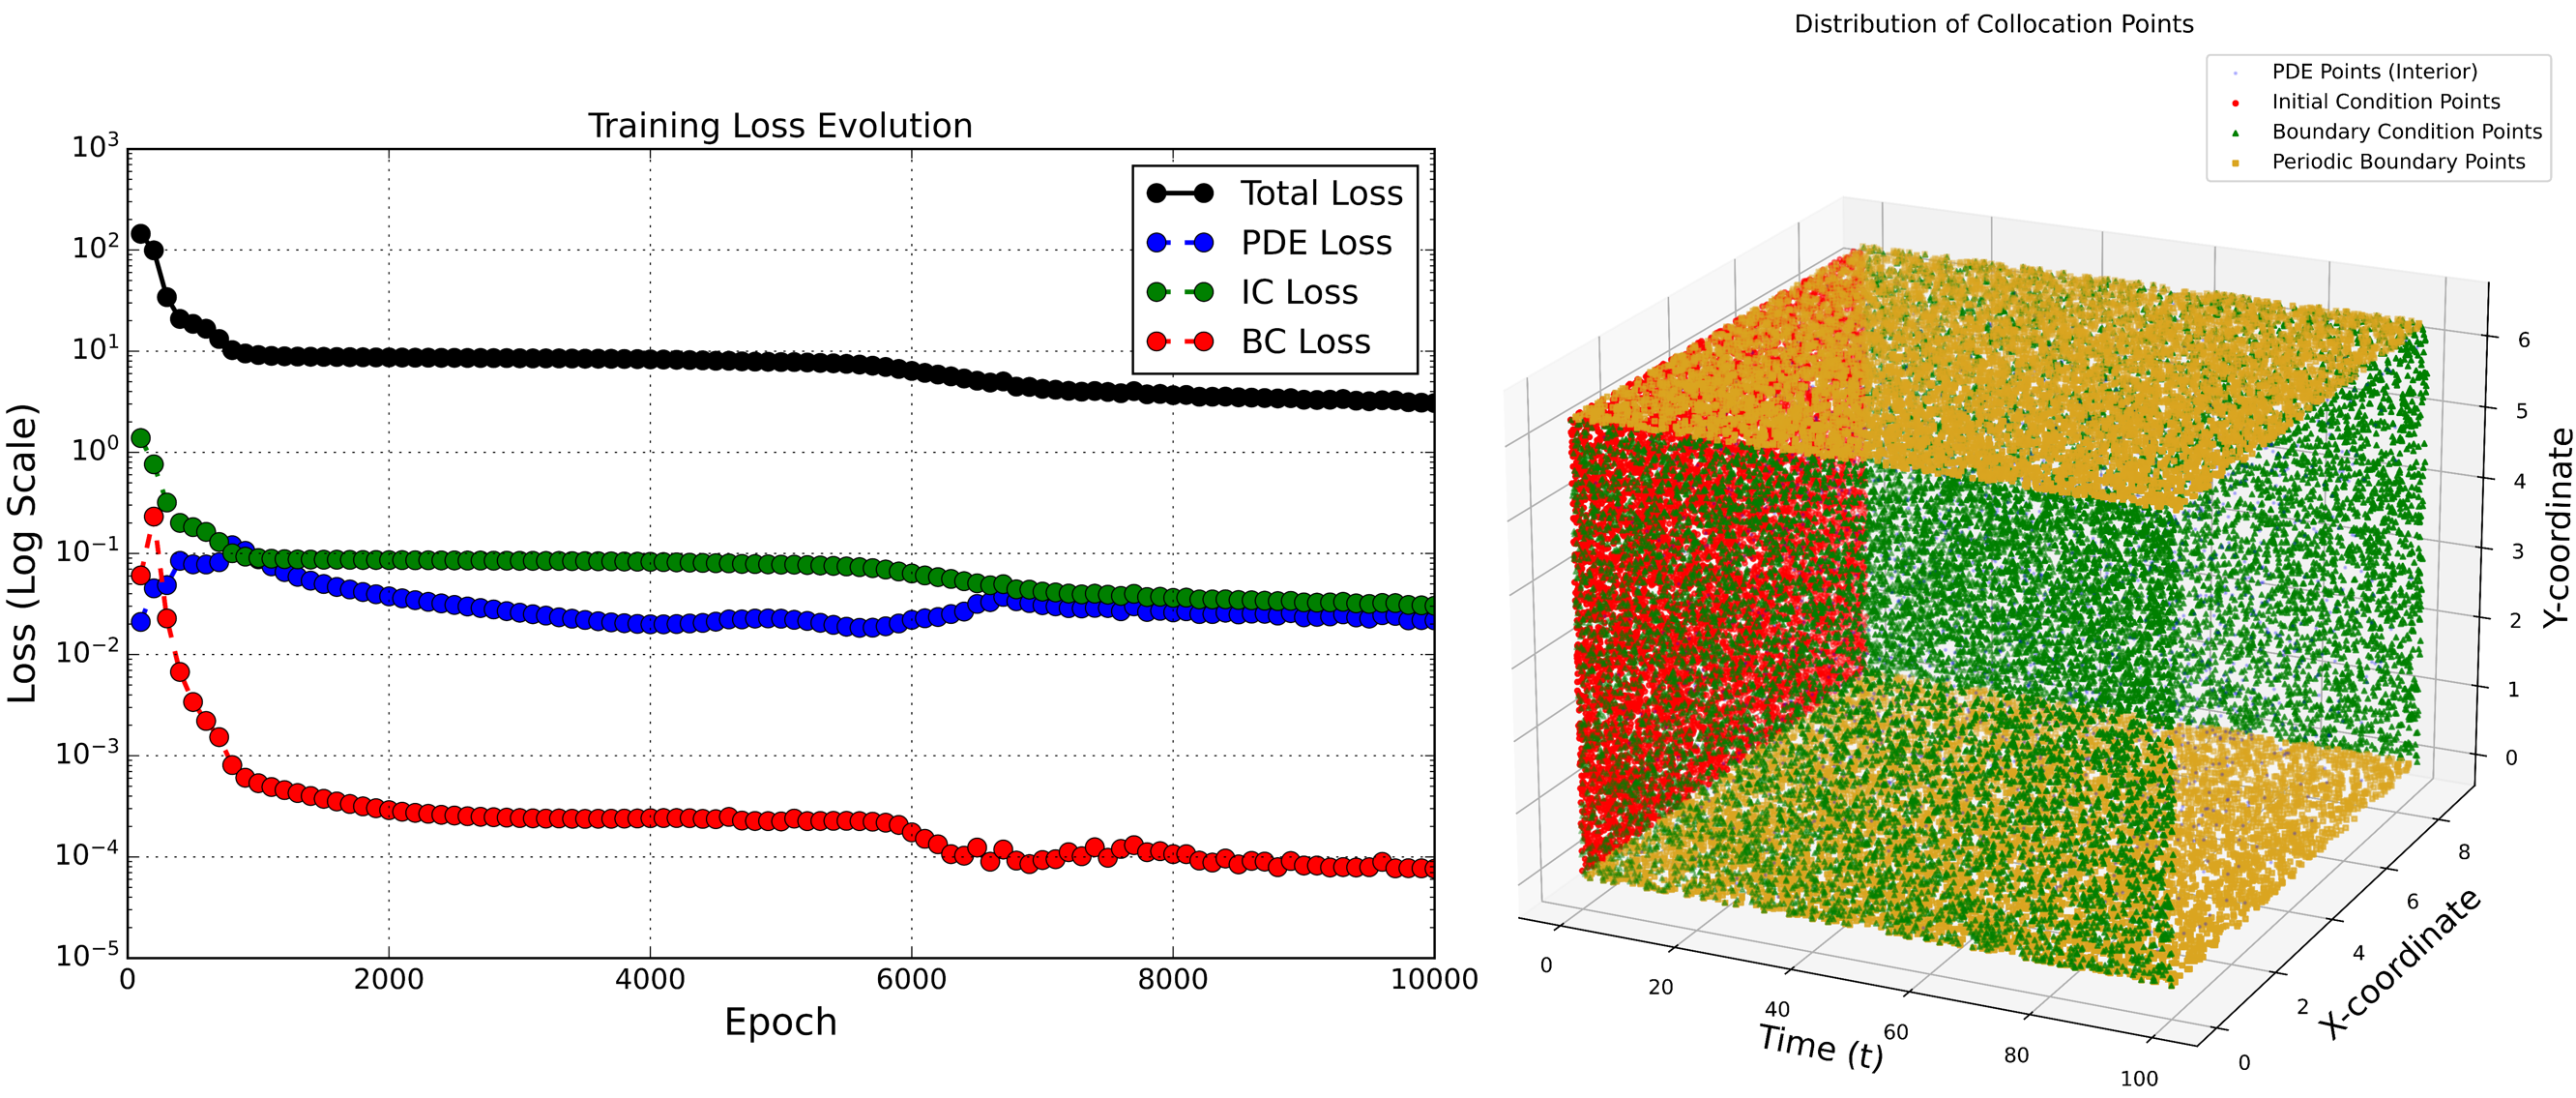
\includegraphics[width=1.0\textwidth]{Figures/IC_loss.png}
    \caption{(left) Evolution of the constituent loss terms (PDE, IC, BC) and Total Loss for the first 10,000 epochs (weights: $\bm{\omega}_\mathrm{PDE} = 1.0$, $\bm{\omega}_\mathrm{IC}, \bm{\omega}_\mathrm{BC} = 100.0$); (right) Initial generation of training (collocation) points, then resampled every 1000 epochs ($N_\mathrm{PDE} = 25,000$: interior points, $N_\mathrm{IC} = 10,000$, $N_\mathrm{BC} = 7500$: both wall and periodic boundaries)}
    \label{fig:IC_loss}
\end{figure}

\section{Verification}

\subsection*{Training and Optimization: \qquad}
The total loss function $\mathcal{L}$ is the weighted sum:
$$ \mathcal{L} = \bm{\omega}_{\mathrm{PDE}} \mathcal{L}_\mathrm{{PDE}} + \bm{\omega}_{\mathrm{IC}} \mathcal{L}_{\mathrm{IC}} + \bm{\bm{\omega}}_{\mathrm{BC}} \mathcal{L}_{\mathrm{BC}} \; .$$
Gradient descent was controlled with the \texttt{Adam} algorithm (Adaptive Moment Estimation) optimizer with an initial learning rate $\sigma = 1 \times 10^{-4}$. The learning rate was then adaptively adjusted for each individual parameter automatically based on the first and second moments of the gradients. A decay factor of 0.9 was applied every 2000 epochs. Initial training (collocation) points, shown in Figure~\ref{fig:IC_loss}, were generated with Latin Hypercube sampling (interior points: $N_\mathrm{PDE} = 25,000$: initial condition points: $N_\mathrm{IC} = 10,000$, wall and periodic boundary points: $N_\mathrm{BC} = 7500$). These points were resampled every 1000 epochs to improve generalization and prevent overtraining. Hyper-parameter tuning of the network (number of hidden layers, neurons, activation functions), optimizer (algorithm, initial learning rate), and scheduler (epoch step size, decay factor) was beyond the scope of this project.
\\ \\
A significant challenge encountered was the optimization landscape. As shown in Figure~\ref{fig:IC_loss}, the IC and BC losses converge rapidly, but the PDE loss plateaus. This indicates the network is ``lazy,'' satisfying the easy boundary constraints while struggling to minimize the complex PDE residuals in the domain interior. To combat this, the loss weights were manually adjusted, reducing $\bm{\omega}_{\mathrm{IC}}$ and $\bm{\omega}_{\mathrm{BC}}$ to encourage the optimizer to focus on the physics. For the first 10,000 epochs: $\bm{\omega}_\mathrm{PDE} = 1.0$, $\bm{\omega}_\mathrm{IC}, \bm{\omega}_\mathrm{BC} = 100.0$. Training weights were adjusted to favor PDE loss ($\bm{\omega}_\mathrm{PDE}, \bm{\omega}_\mathrm{IC}, \bm{\omega}_\mathrm{BC} = 10.0$) after 10,000 epochs. Verification of the PINN was performed by monitoring the loss convergence. Figure~\ref{fig:loss_evo} displays the full loss history. The rapid drop in BC loss confirms the network satisfies the periodicity and wall conditions. The slow decay of the PDE loss suggests the network is resolving the mean flow but struggling with smaller scales.

\subsection*{Computational Cost: \qquad}
Both the \texttt{PyTorch} and \texttt{Miranda} codes are written for CPU and GPU (\texttt{Cuda}) portability. CPU runs were completed on \texttt{CZ} \texttt{DANE} with Intel Sapphire Rapids (Xeon(R) Platinum 8480+) 112 cores/node architecture. GPU acceleration was achieved on \texttt{Adroit} with NVIDIA A100 GPUs (4 per node), in addition to the same Intel Sapphire Rapids CPU node.
\begin{itemize}
    \item \textbf{PINN:} Training required approximately 100,000 epochs, as shown in Figure~\ref{fig:loss_evo}. On CPU, this corresponds to roughly 60-80 hours of wall-time. On GPU an $\approx 10 \times$ speedup was achieved, with training in 6-8 hours. The cost is dominated by the automatic differentiation graph traversal for derivatives. Inference time for figure generation was negligible.
    \item \texttt{Miranda:} The finite-difference solver ran on the same domain with a coarse $256 \times 256$ grid. While explicit time-stepping requires many steps, the per-step cost is low. For this 2-D problem, \texttt{Miranda} is orders of magnitude faster (minutes vs. hours) than training the PINN.
\end{itemize}
The mesh-free paradigm of PINNs allows for a computational cost independent of resolution once training is complete. Inference time for figure generation will increase with resolution, but still on the order of minutes. Scaling of compressible finite-difference codes is prohibitive ($\propto N_\mathrm{pts}^3$ in 2-D, inclusive of timestep stability; $\propto N_\mathrm{pts}^4$ in 3-D).

\section{Application}

\subsection*{Comparison with \texttt{Miranda} (iLES): \qquad}
Results are shown for the trained PINN applied to the evolution of RTI for $t \in [0,100]$ [sec]. This is sufficient time for a well developed mixing layer such that $t_\mathrm{max} / \tau_0 > 10$. The specified resolution for both the PINN and \texttt{Miranda} benchmark was $N_{\mathrm{pts}}=256$.
\\ \\
Figure~\ref{fig:time_evo} shows time evolution of the density field computed from \texttt{Miranda}. The fine scale turbulent structures can be seen clearly. This includes the secondary Kelvin-Helmholtz instabilities that create the ``roll-up'' on the sides of the mushroom cap, the secondary vortices, and the eventual chaotic mixing at the smallest scale with highly localized mixed regions at the interface. The progression from early linear growth, non-linear saturation (bubble and spike formation), and late-time mixing can be closely delineated.
\\ \\
A comparison of the initial conditions from the PINN and \texttt{Miranda} is shown in Figure~\ref{fig:ic_field} for the density field and flow parameters vertically averaged in $y$. The analytical solution and diffuse interface for pressure, density, and mass fraction implemented in \texttt{Miranda} is also shown. A comparison of the density field shows a close match of the interface, though there is significant dispersion in the diffuse region. This can also be seen in the mixing ratio ($\theta \in \left[0,1\right]$, $\theta = 0$ fully segregated, $\theta = 1$ fully mixed), which is initially not sharp.

\begin{landscape}
\begin{figure}[h!]
    \centering
    \vspace{-0.5cm}
    \includegraphics[width=0.88\textwidth]{Figures/Loss_Evolution.png}
    \caption{Evolution of the constituent loss terms (PDE, IC, BC) and Total Loss over 100,000 epochs. Note the rapid convergence of BCs contrasted with the slow, plateauing decay of the PDE loss, indicative of the optimization difficulty in the domain interior. Training points were resampled every 1000 epochs for generalization; training weights were adjusted to favor PDE loss ($\bm{\omega}_\mathrm{PDE}, \bm{\omega}_\mathrm{IC}, \bm{\omega}_\mathrm{BC} = 10.0$) after 10,000 epochs.}
    \label{fig:loss_evo}
\end{figure}
\begin{figure}[h!]
    \centering
    \vspace{-0.5cm}
    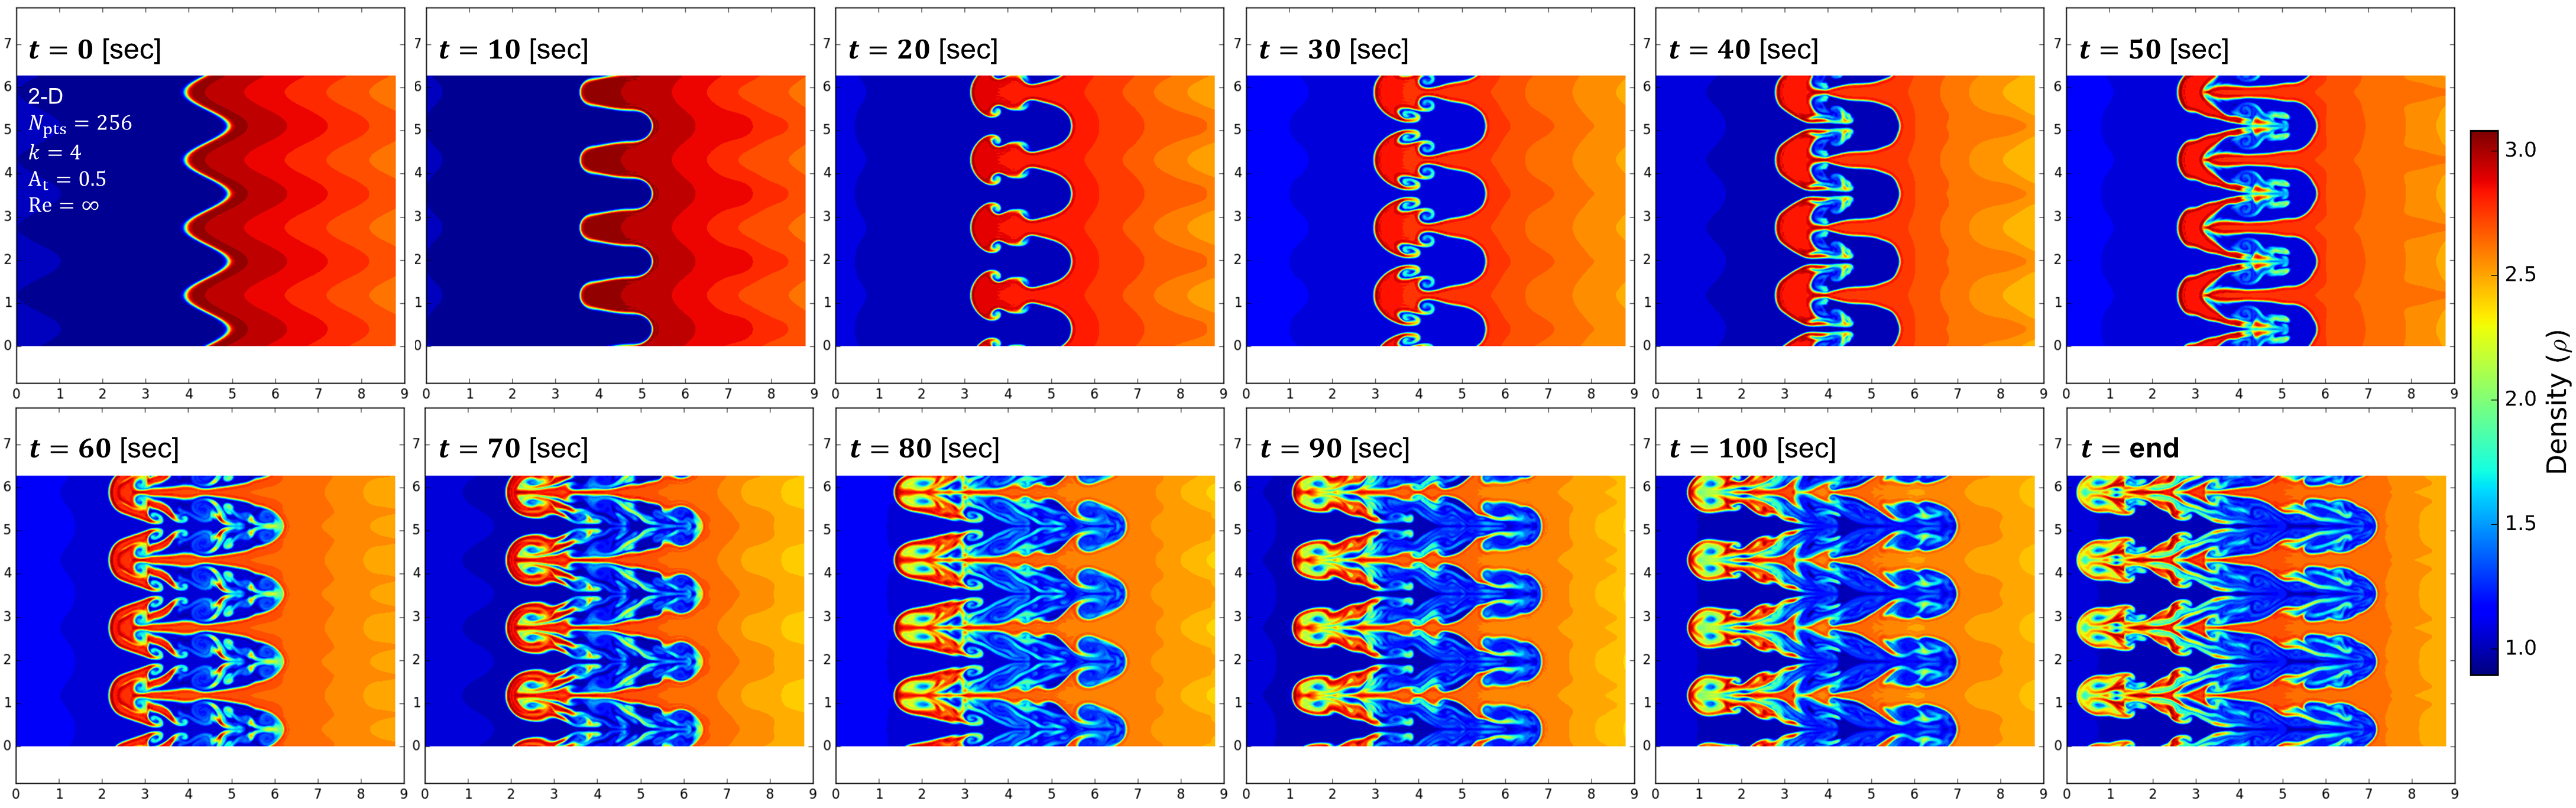
\includegraphics[width=1.36\textwidth]{Figures/time_evolution_picture_med-res.png}
    \caption{Time evolution of the density field computed from \texttt{Miranda}, showing the progression from early linear growth, non-linear saturation (bubble and spike formation), and late-time mixing.}
    \label{fig:time_evo}
\end{figure}
\end{landscape}

The mixing ratio in time $\theta\left(t\right)$ can be expected to grow as:
$$\theta(t) = \frac{\int\overline{Y_h} \left(1-\overline{Y_h}\right) \, \mathrm{d} x}{\int\overline{Y_h(1-Y_h)} \, \mathrm{d} x} = 1 - \frac{4\int\overline{Y_h Y_\ell} \, \mathrm{d} x}{h(t)} \; .$$
$\overline{(\cdot)}$ is the ensemble mean (2-D average in height). The mixing layer width $h = C_h \int_{0}^{L_x}{\overline{Y_h}\left(1-\overline{Y_h}\right) \mathrm{d} x}$ is defined up to a multiplicative normalization factor $C_h = 4$ for a diffuse interface. Figure~\ref{fig:snapshots} shows the instantaneous profiles of the flow variables every $t=10$ [sec] from \texttt{Miranda} and the final value captured by the PINN. Figure~\ref{fig:comparison} shows the predicted pressure field with velocity vectors and vorticity field ($\omega = \nabla \times \mathbf{u}$) at PINN initialization and end. In summary:
\begin{itemize}
    \item \textbf{Mean Flow:} The PINN accurately captures the position of the bubble and spike tips. The global symmetry and stratification are preserved.
    \item \textbf{Turbulence and Spectral Bias:} A stark difference is visible in the resolution of fine structures. The \texttt{Miranda} simulation (Figure~\ref{fig:time_evo}) shows Kelvin-Helmholtz roll-up and secondary vortices. The PINN solution (Figure~\ref{fig:comparison}) appears highly diffused. The vorticity field highlights the shear layers at the bubble-spike interface. The lack of small-scale vortices indicates the spectral bias filtering high-frequency dynamics. This confirms the hypothesis of spectral bias; the neural network acts as a low-pass filter, effectively simulating a flow with a much higher effective viscosity.
\end{itemize}

\begin{figure}[h!]
    \centering
    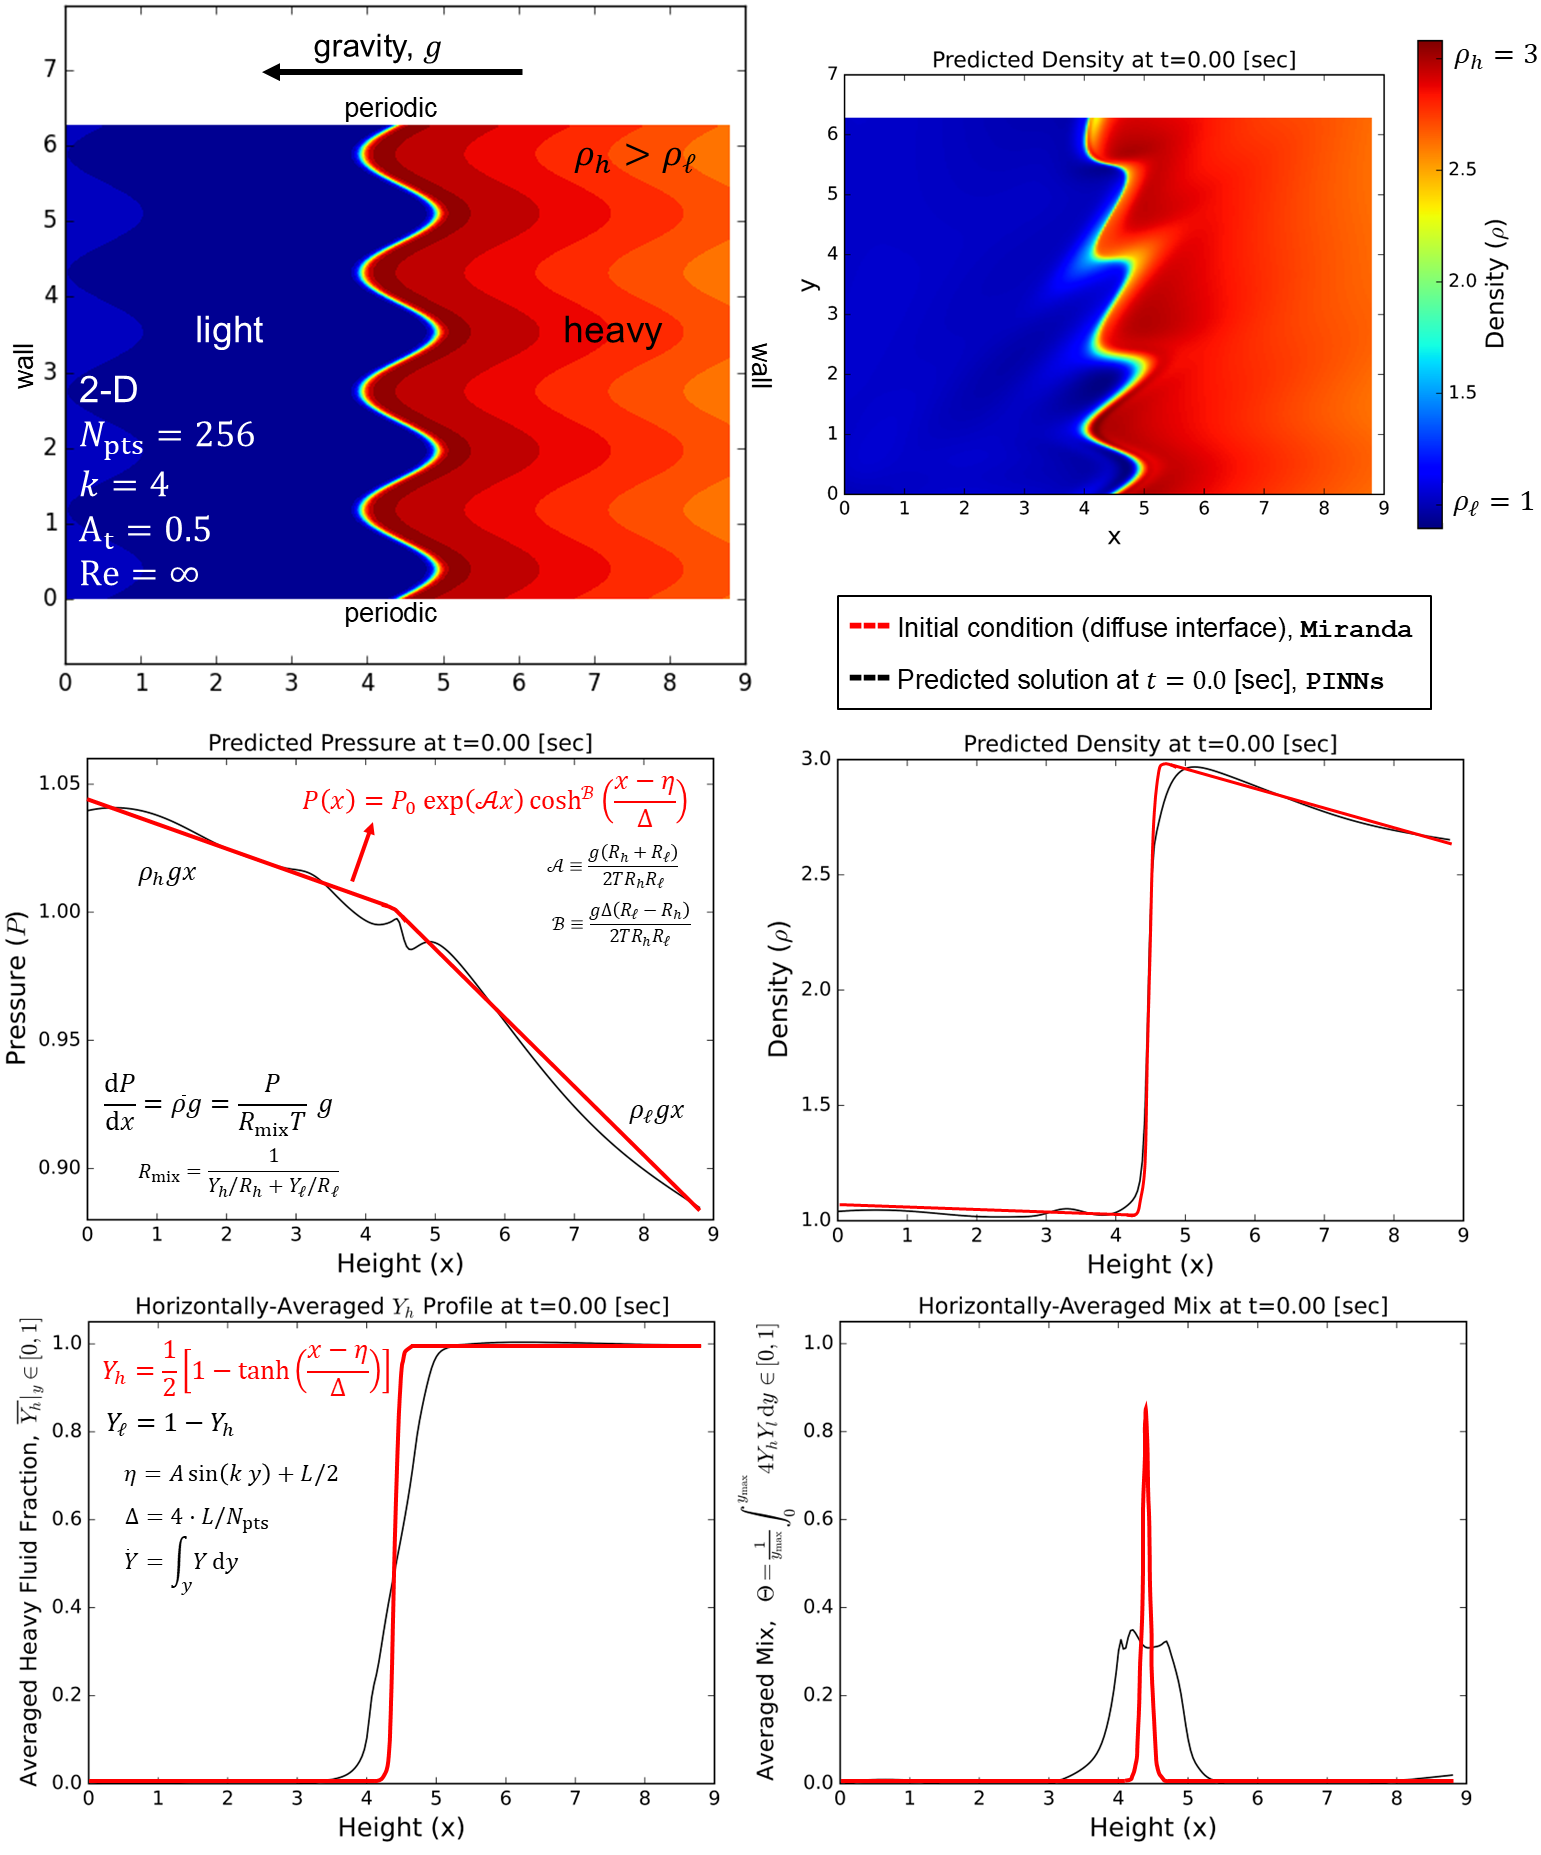
\includegraphics[width=0.8\textwidth]{Figures/initial_med-res.png}
    \caption{Initial conditions for the Rayleigh-Taylor instability simulation. Initial \texttt{Miranda} values (red lines) for pressure and fluid mass fraction are determined from the ideal gas law and hydrostatic equilibrium, shown in the figures as a function of height $x$. Predicted PINNs solution at $t = 0$ [sec] is shown with black lines. The density field shows the heavy fluid (red, left) and light fluid (blue, right) separated by a perturbed interface.}
    \label{fig:ic_field}
\end{figure}

\begin{figure}[h!]
    \centering
    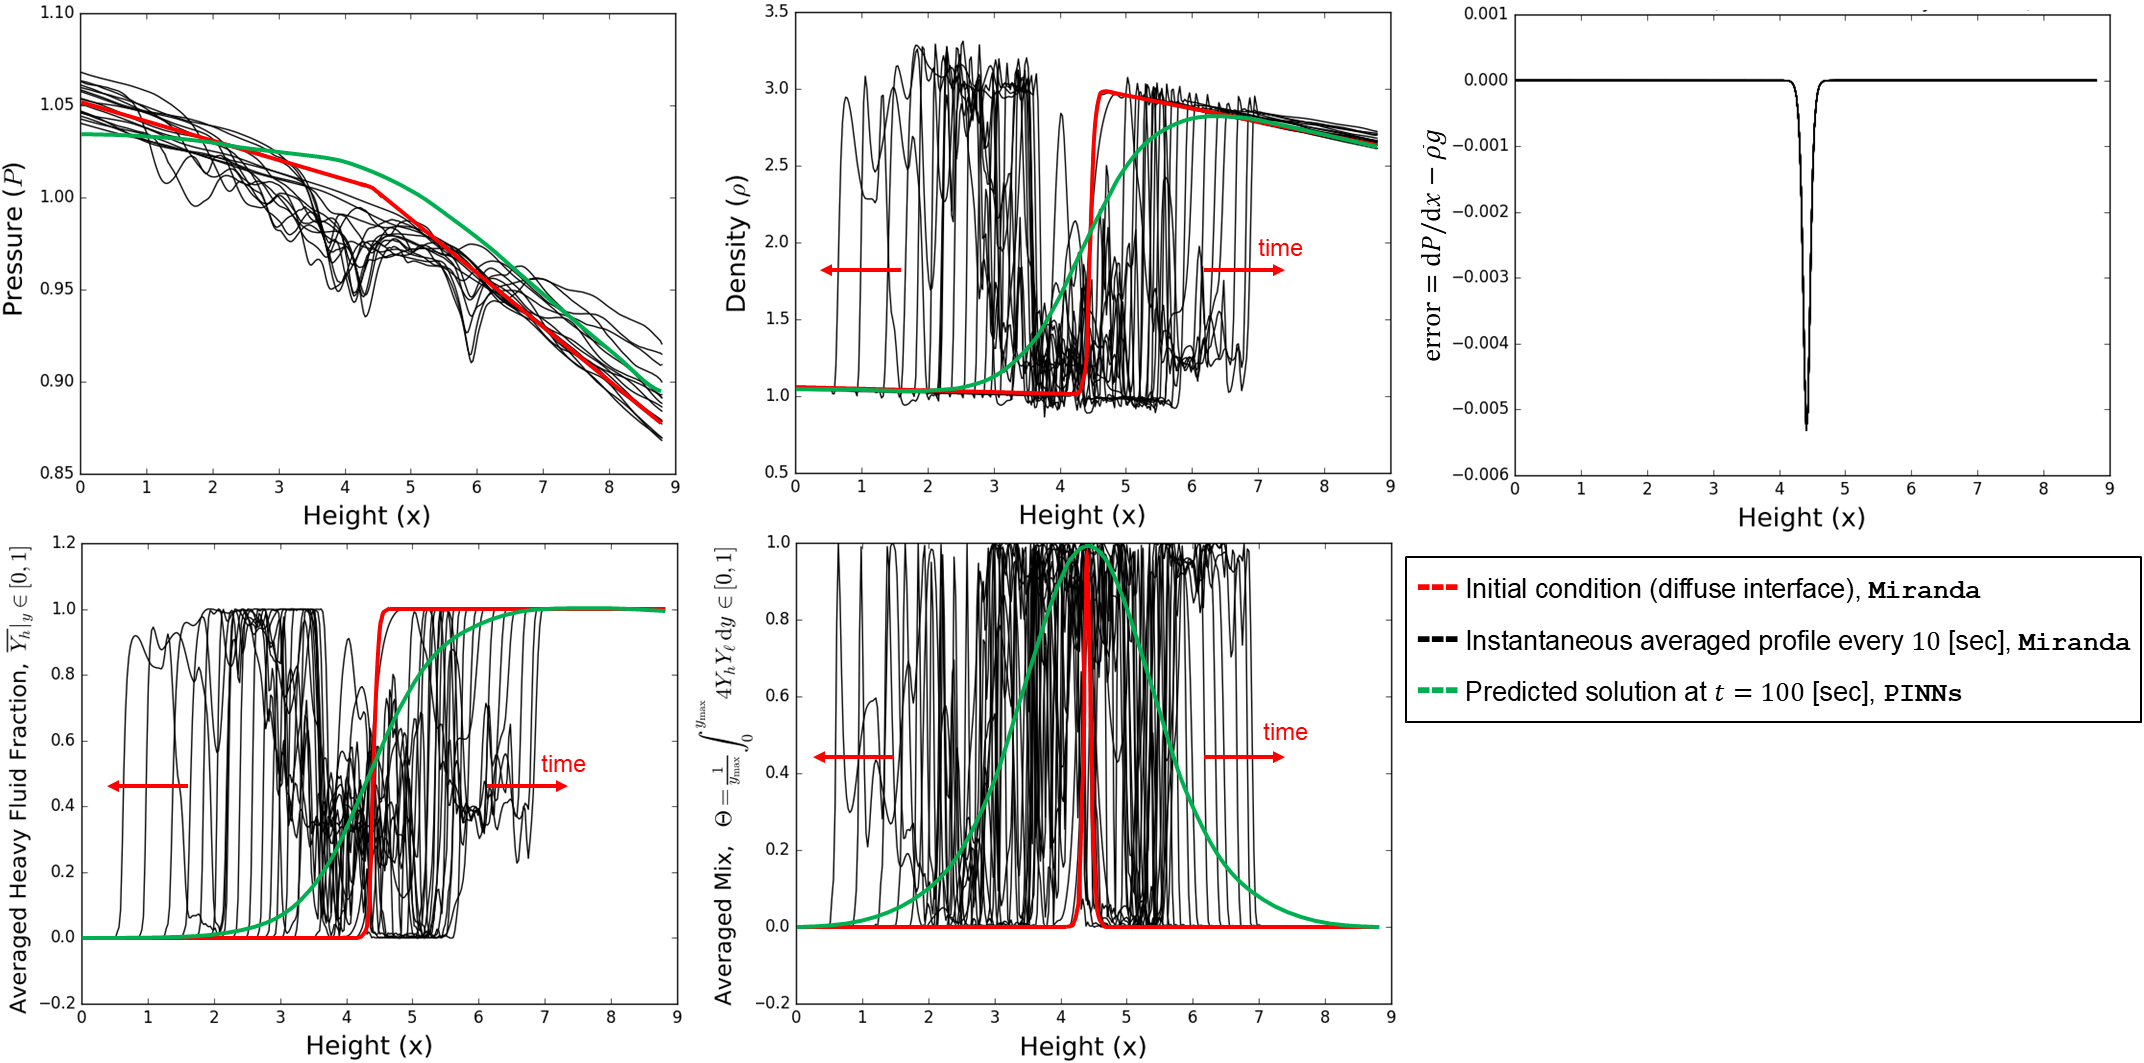
\includegraphics[width=1.03\textwidth]{Figures/time_evolution_med-res.png}
    \caption{Instantaneous profiles of mixture and flow variables vertically averaged over the domain. Black lines show the broadening of the mixing layer in time. With the PINN's prediction (green) at late time, the interface remains coherent but highly diffusive, characteristic of a low-Reynolds number flow or a RANS-like approximation.}
    \label{fig:snapshots}
\end{figure}

\begin{figure}[h!]
    \centering
    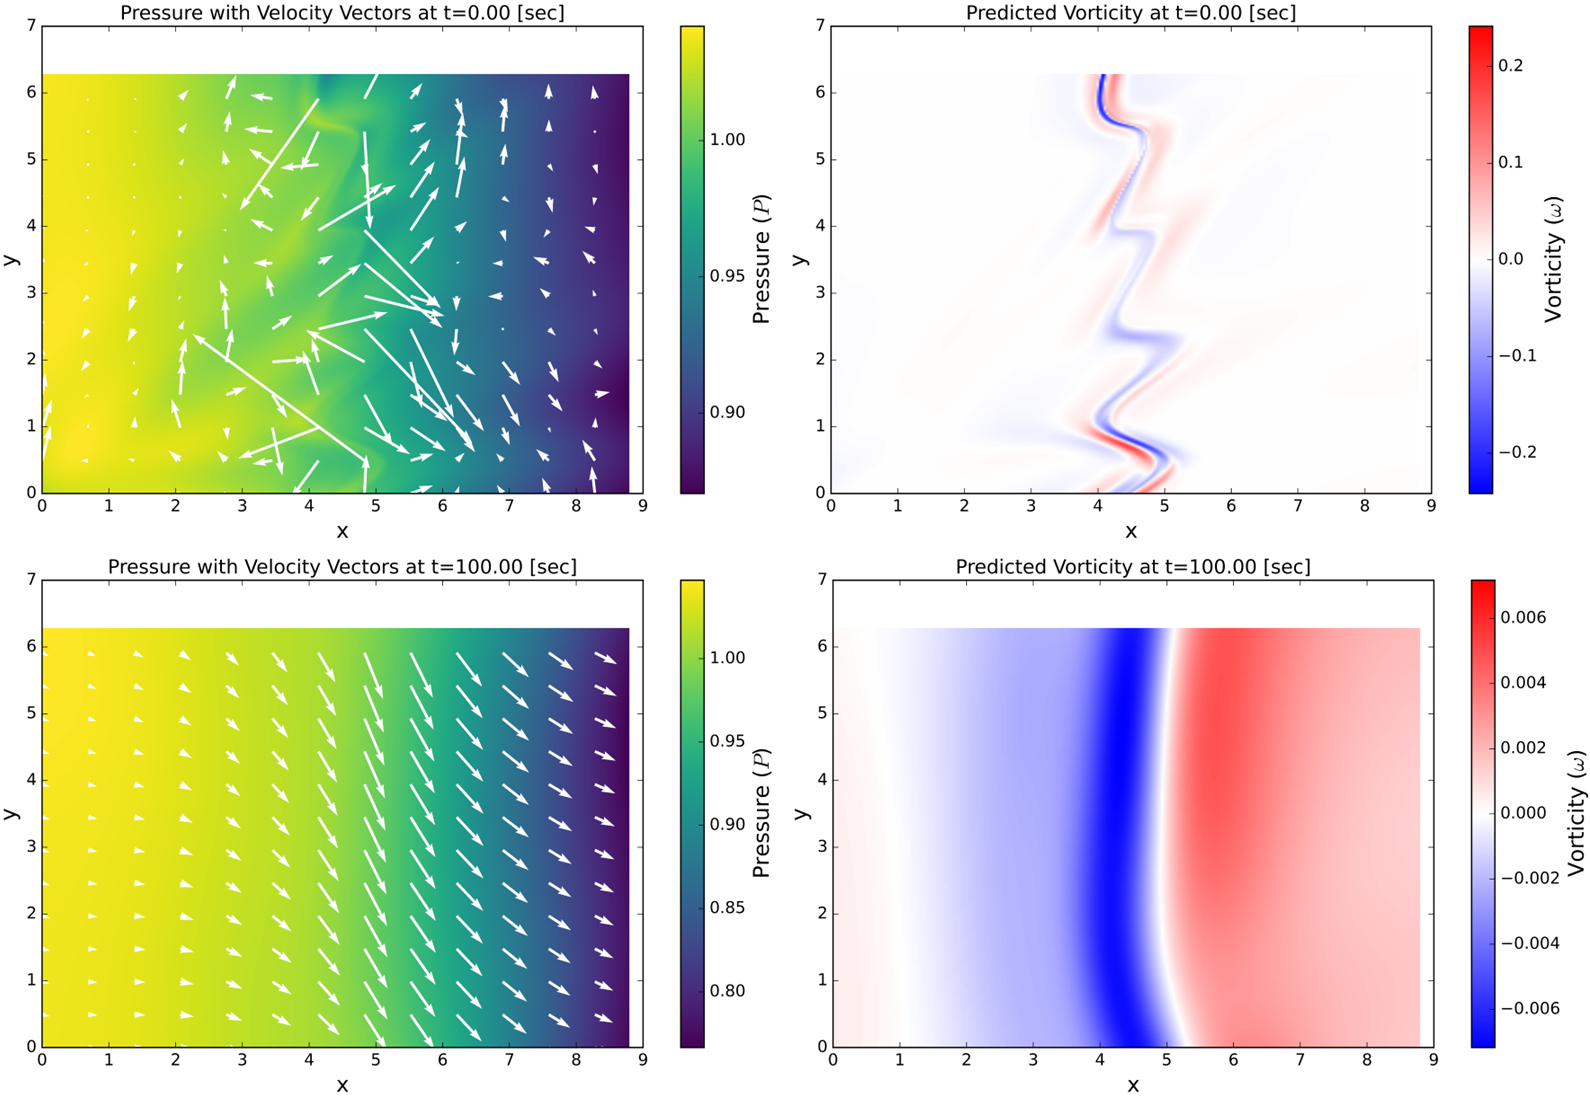
\includegraphics[width=0.85\textwidth]{Figures/Pressure_Vorticity_med-res.png}
    \caption{Predicted Pressure field with velocity vectors (left) and Vorticity field (right) at PINN initialization ($t = 0$ [sec]) and end ($t = 100$ [sec]). The vorticity field highlights the shear layers at the bubble-spike interface. The lack of small-scale vortices indicates the spectral bias filtering high-frequency dynamics.}
    \label{fig:comparison}
\end{figure}

\subsection*{Characteristics of the Bulk Flow: \qquad}
While the PINN struggles to capture small-scales structures, macroscopic parameters like the mixing layer thickness and growth rate are also of interest. The mixing layer width $h = 4 \int\overline{Y_h} \left(1-\overline{Y_h}\right) \mathrm{d} x$ has been shown \cite{Ristorcelli2004,Cook2004} to theoretically grow, 
$$h(t) = \alpha \mathrm{A_t} g t^2+2t\sqrt{\alpha \mathrm{A_t} g h_0}+h_0 \; ,$$
with a growth rate $\dot{h}(t)=\sqrt{4\alpha \mathrm{A_t} g t^2}$. $\alpha$ [-] is a ``self-similarity'' parameter that settles to a constant in fully developed turbulence. The mixing width $h(t)$ is shown in Figure~\ref{fig:mixing_width}. The PINN prediction roughly follows the theoretical quadratic growth $h \approx \alpha \mathrm{A_t} g t^2$, confirming that the solver is capturing the fundamental driving force of the instability.

\begin{figure}[h!]
    \centering
    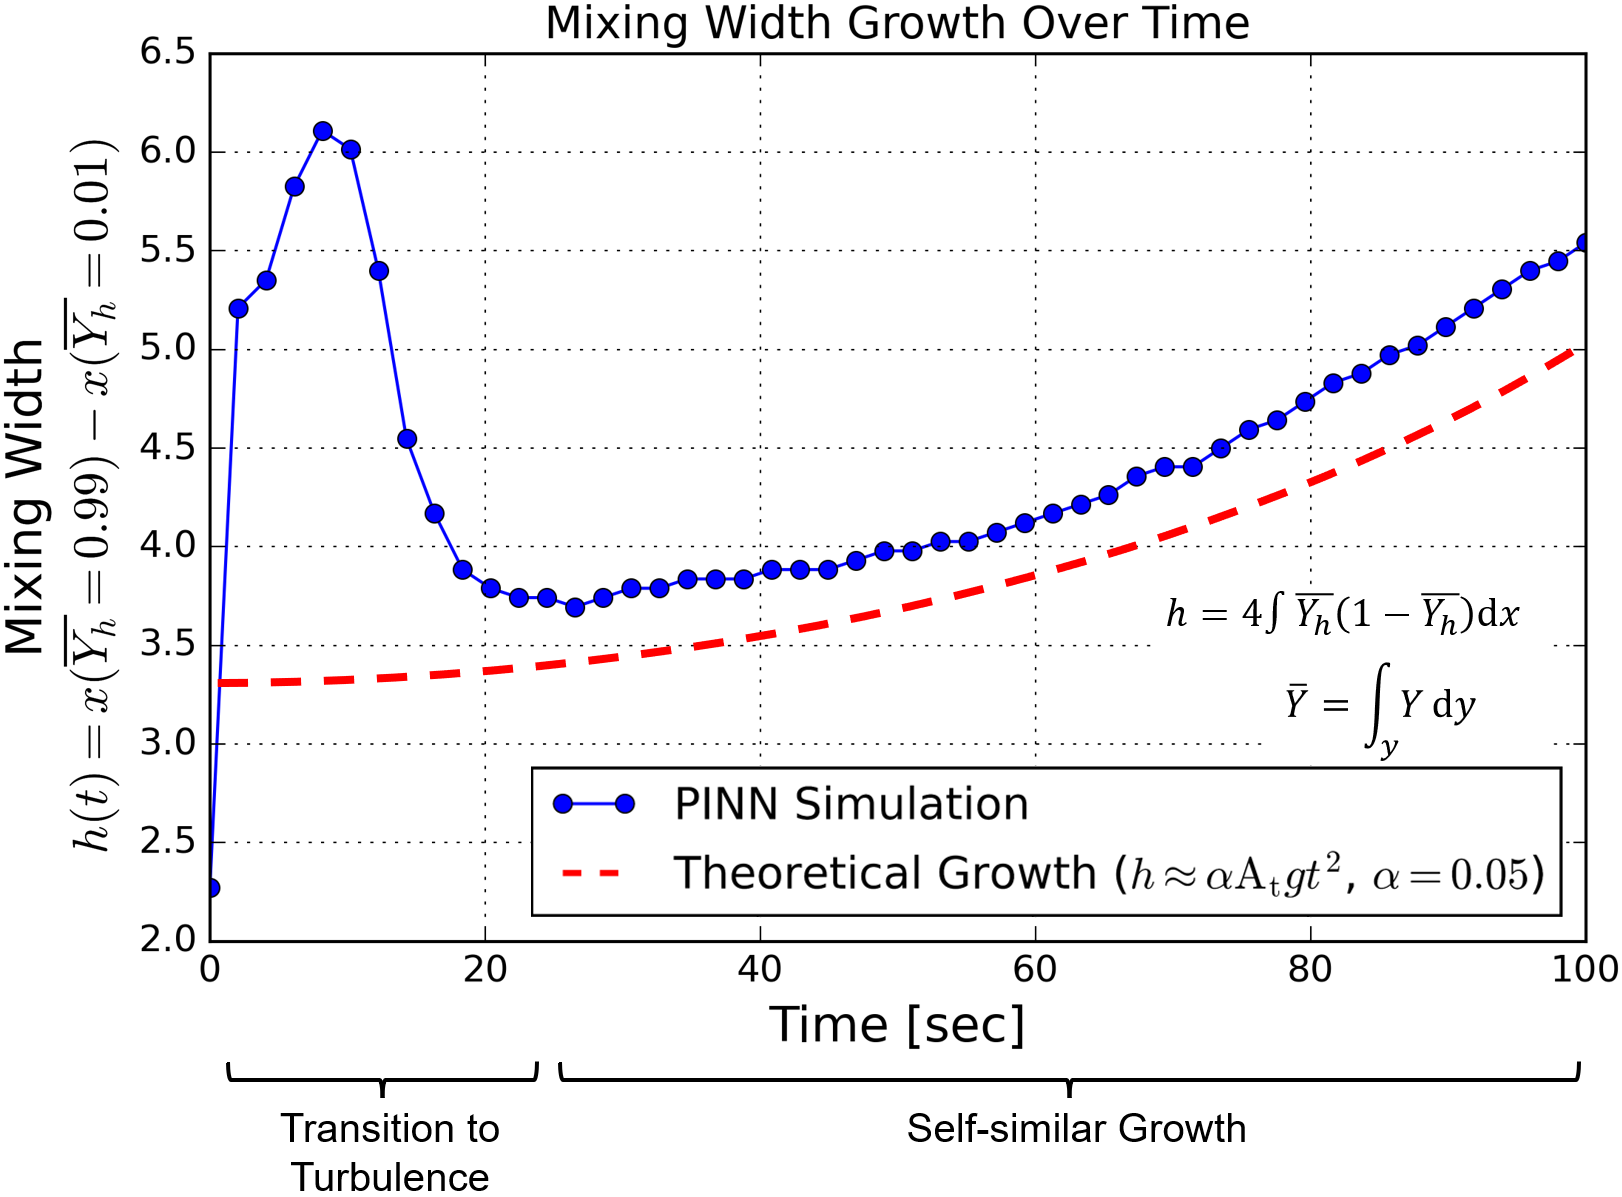
\includegraphics[width=0.6\textwidth]{Figures/Mixing_Width.png}
    \caption{Evolution of the mixing width $h(t)$ predicted by the PINN compared to the theoretical quadratic growth $h \sim t^2$. The agreement in the growth trend validates the PINN's ability to capture the bulk mixing rate.}
    \label{fig:mixing_width}
\end{figure}

\subsection*{Discussion of Failure Modes: \qquad}
The ``smoothness'' of the PINN solution is not merely a resolution issue but a fundamental property of the training dynamics. The high-frequency components of the solution (turbulence) correspond to small eigenvalues in the Neural Tangent Kernel (NTK) \cite{Rahaman2019,LUO2021}, meaning they are learned exponentially slower than low-frequency components. The standard fully-connected architecture used here inherently behaves like a Reynolds-Averaged model, capturing the mean profile while filtering fluctuations.
\\ \\
Several effective techniques have been developed to help PINNs learn high frequencies. \emph{Fourier Feature Mapping} \cite{Tancik2020,WANG2021} is a feature engineering approach that transforms the raw inputs into a higher-dimensional feature vector containing sine and cosine terms of increasing frequencies $[\sin(k\,x), \sin(2k\,x),\dots]$. This essentially converts a high-frequency problem into a low-frequency problem that the network is much better at learning. Some specialized network architectures are inherently better at representing high-frequency details. \emph{SIRENs (Sinusoidal Representation Networks)}, which use $\sin(x)$ as their activation function, are a prime example. \emph{Adaptive Sampling} periodically checks where the PDE error is highest and adds more training points to those ``difficult'' regions, rather than sampling collocation points randomly. This forces the network to pay more attention to the areas where high-frequency structures are forming. Similarly \emph{Adaptive Activation Functions} \cite{JAGTAP2020} may select the network activation function in high error regions. \emph{Curriculum Learning} trains the network in stages, starting with an ``easy'' version of the problem (e.g., low Reynolds number or a short time duration where the flow is still smooth). Then, it uses those trained weights as a starting point to continue training on the harder, more turbulent version of the problem. \emph{Cyclical Learning Rates} use a scheduler (\texttt{torch.optim.lr\_scheduler.CyclicLR} in \texttt{PyTorch}) that varies the learning rate up and down between a minimum and maximum value over a set number of epochs. The ``uphill'' part of the cycle is designed specifically to escape local minima.
\\ \\
Hyper-parameter tuning (via Bayesian optimization) of the network architecture (number of hidden layers, neurons, activation functions), optimizer (algorithm, initial learning rate), and scheduler (epoch step size, decay factor) was beyond the scope of this project. If the network is too shallow or narrow, it may not have the capacity to represent the complex solution to the Navier-Stokes equations. It may be advantageous to make the network deeper (e.g., 10 layers instead of 8) or wider (e.g., 256 neurons instead of 128). While loss function weights were changed manually to favor PDE loss later in training, optimizations can be further implemented to change the loss weights dynamically. 

\section*{Conclusion}
This project successfully developed a PINN solver for the 2-D compressible Navier-Stokes equations and applied it to the Rayleigh-Taylor instability. Comparison with the high-order \texttt{Miranda} code revealed that while PINNs can accurately enforce boundary conditions and capture macro-scale dynamics (linear growth rates, mixing width), they struggle significantly with the high-frequency spectrum required for turbulence. The PINN solution resembles a highly viscous or ensemble-averaged flow. Future work to make PINNs viable for DNS/LES of turbulence must incorporate spectral bias mitigation strategies, such as Fourier features or multi-scale network architectures.

\section*{Supplement}
The core code libraries for the results presented are available at the following repository, including instructions for running and compiling (primarily in \texttt{Jupyter} notebook).
\\ \\
Github: \href{https://github.com/mw6136/RT-PINNs}{https://github.com/mw6136/RT-PINNs}

\bibliographystyle{plain}
\bibliography{citations.bib}

\appendix
\section*{Appendix}
\section{Network Structure Visualization}
Figure~\ref{fig:NN_struct} shows the deep feed-forward neural network structure. Figure~\ref{fig:pinn_struct} shows a full backward pass through the neural network. Hyper-parameter tuning of the network (number of hidden layers, neurons, activation functions), optimizer (algorithm, initial learning rate), and scheduler (epoch step size, decay factor) was beyond the scope of this project.
\begin{figure}[h!]
    \centering
    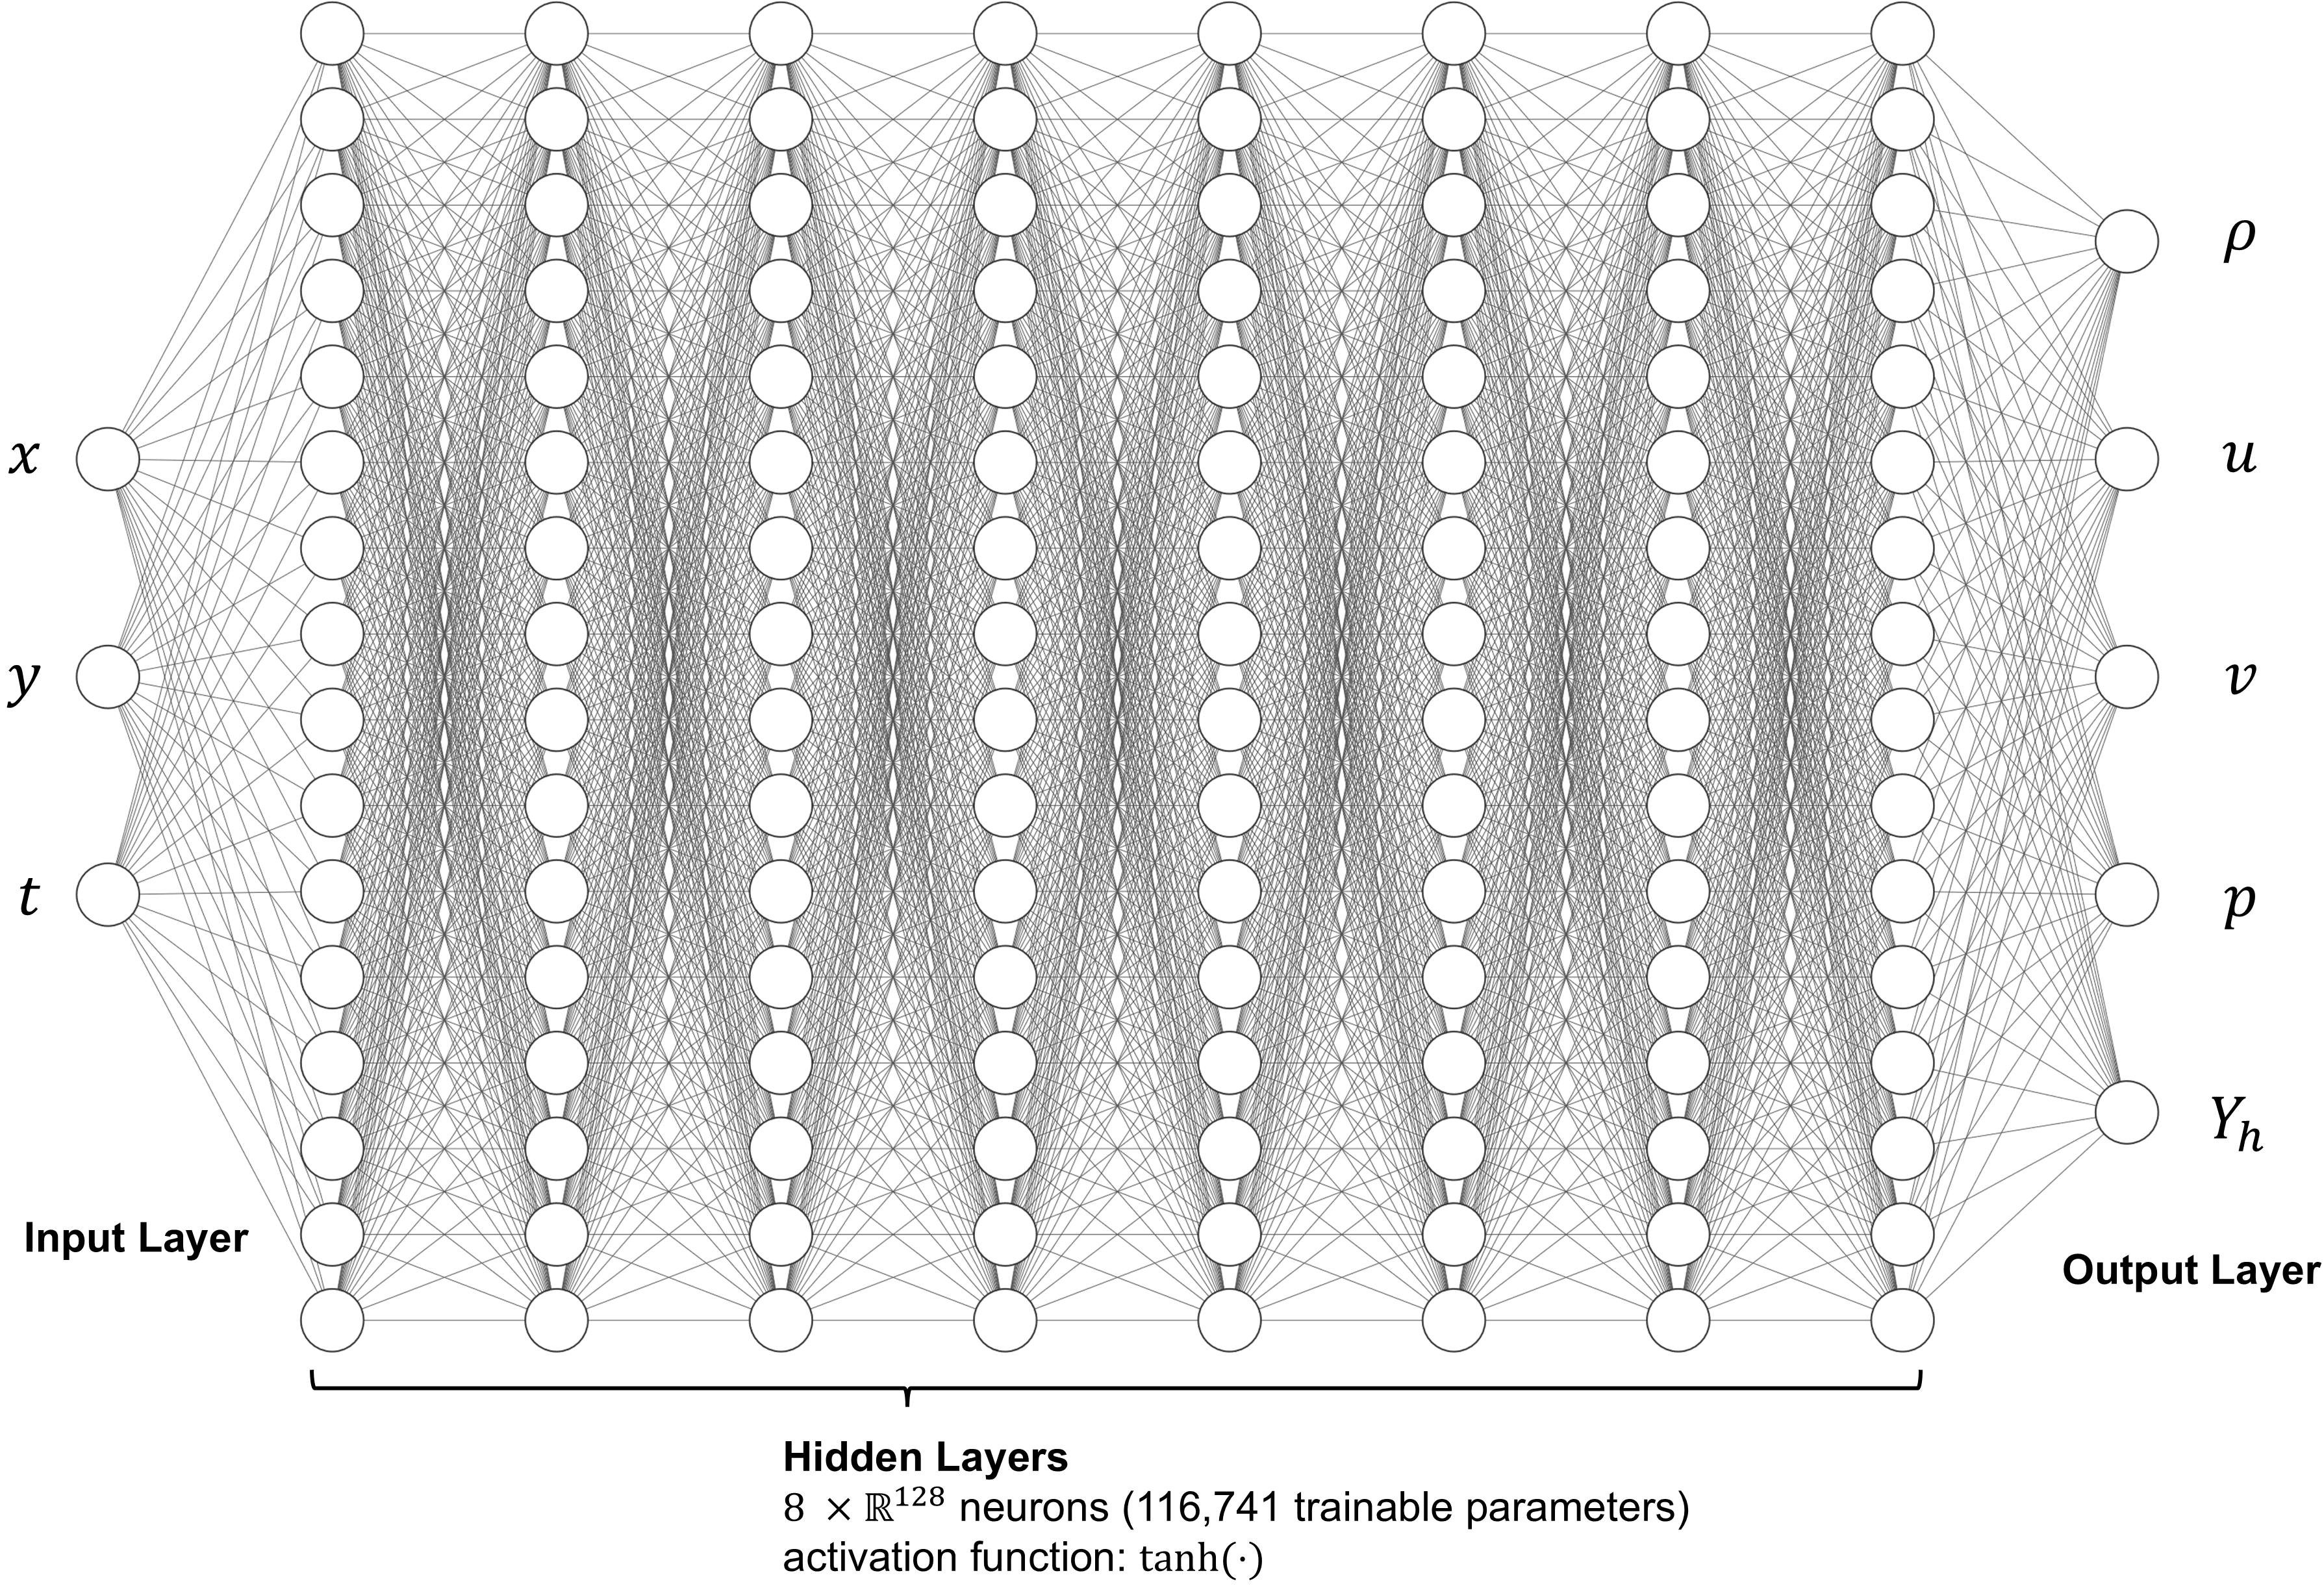
\includegraphics[width=0.77\textwidth]{Figures/NN_med-res.png}
    \caption{Neural Network structure, showing the hidden layers transforming inputs $(t, x, y)$ to flow variables.}
    \label{fig:NN_struct}
\end{figure}

\begin{figure}[h!]
    \centering
    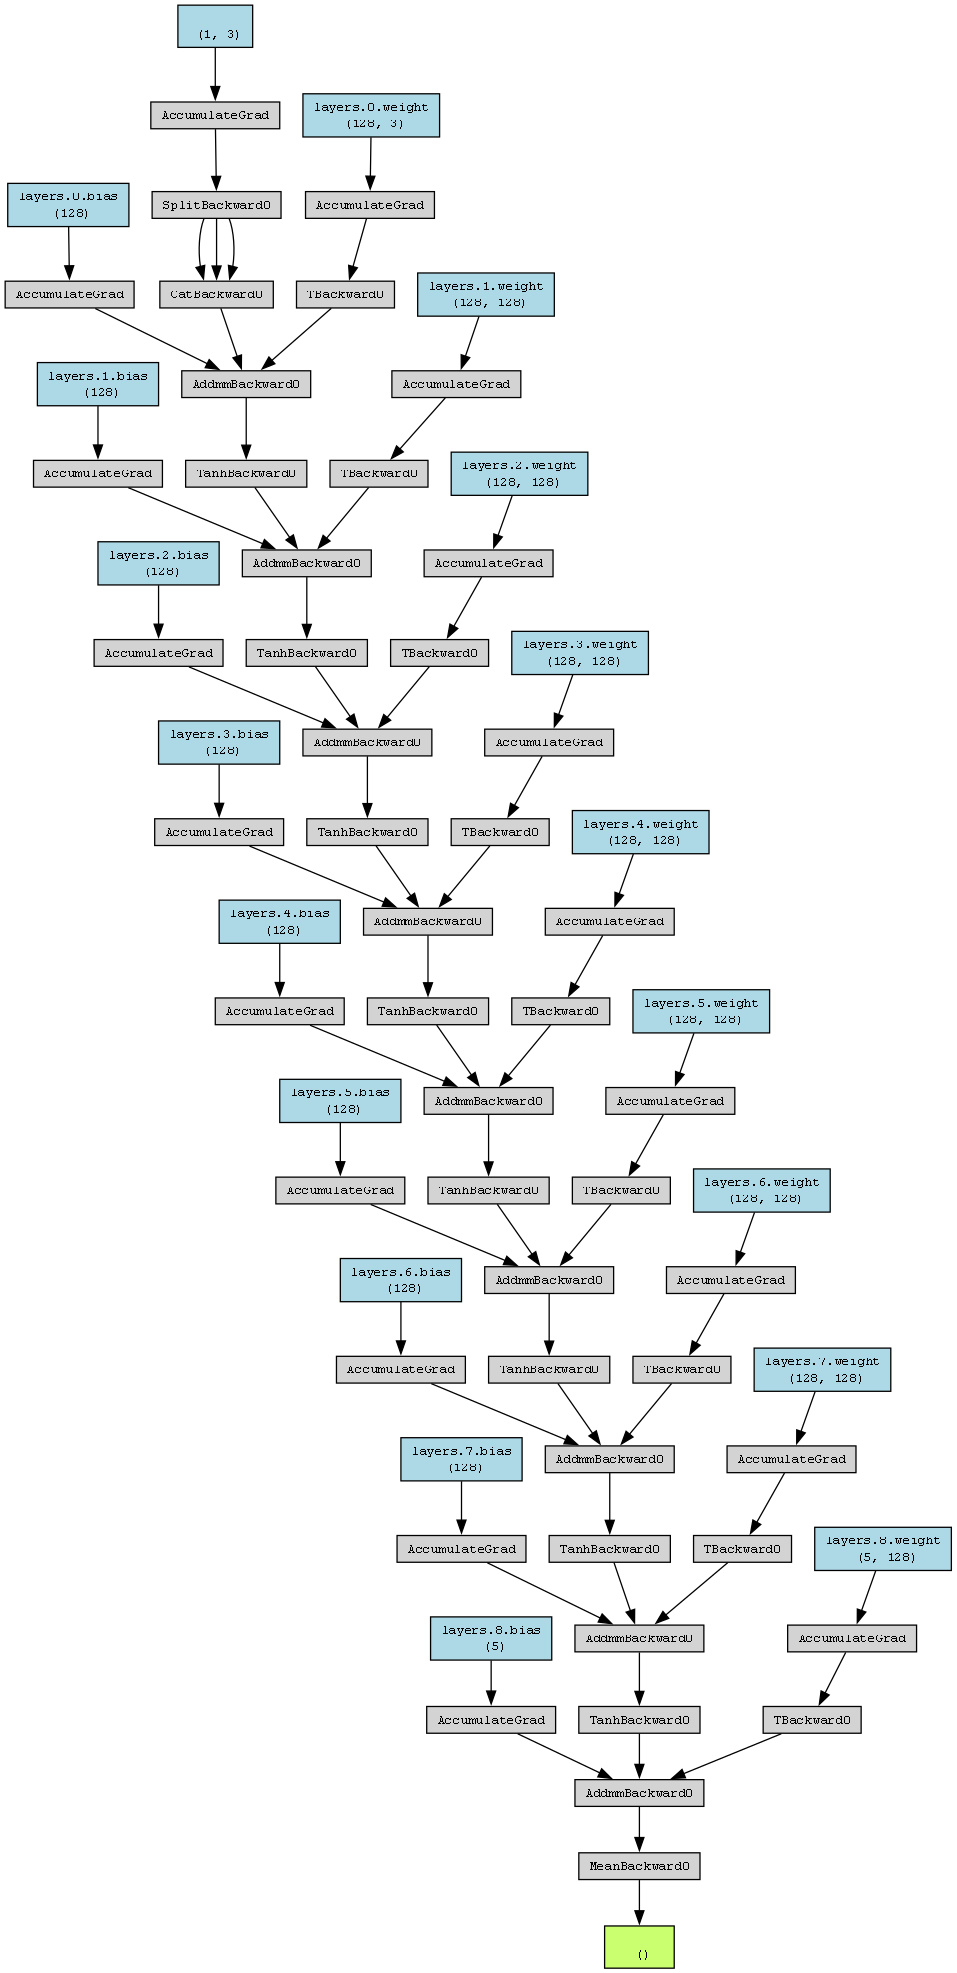
\includegraphics[width=0.61\textwidth]{Figures/pinn_structure.png}
    \caption{Graph visualization of the Physics-Informed Neural Network architecture, showing the fully connected layers transforming inputs $(t, x, y)$ to flow variables.}
    \label{fig:pinn_struct}
\end{figure}

\section{Inclusion of Viscosity}
A PINNs inclusive of viscosity ($\mathrm{Re}=\mathrm{finite}$) and heat flux was developed. Due to the already significant spurious, artificial viscosity present in the inviscid case, the results are not shown. A Reynolds number ($\mathrm{Re} \equiv \rho \lambda_0 \sqrt{g \lambda_0} / \mu$) and Prandtl number ($\mathrm{Pr} \equiv \mu c_p / \kappa \approx 0.71$ for air-like gas) must now be specified to define the dynamic viscosity $\mu$ and thermal conductivity $\kappa$. There is no species diffusion in this model. First, the shear stress and heat flux terms are calculated:
{\small \begin{align*}
    \tau_{xx} &= \tfrac{2}{3} \mu (2 \tfrac{\partial u}{\partial x} - \tfrac{\partial v}{\partial y}) \qquad q_x = -\kappa \, \partial T /\partial x \\
    \tau_{yy} &= \tfrac{2}{3} \mu (2 \tfrac{\partial v}{\partial y} - \tfrac{\partial u}{\partial x}) \qquad q_y = -\kappa \, \partial T /\partial y \\
    \tau_{xy} &= \mu (\tfrac{\partial u}{\partial y} + \tfrac{\partial v}{\partial x})    
\end{align*}}
Then the residuals are calculated for the 5 conservation laws:
{\footnotesize \begin{align*}
    \mathrm{Mass:} \quad &\frac{\partial \rho}{\partial t} + \frac{\partial \rho u}{\partial x} + \frac{\partial \rho v}{\partial y} = 0 \\
    f_\mathrm{mass} &= \left[ \tfrac{\partial \rho}{\partial t} + \tfrac{\partial \rho u}{\partial x} + \tfrac{\partial \rho v}{\partial y} \right] \\
    \mathrm{Species:} \quad &\frac{\partial \rho Y_h}{\partial t} + \frac{\partial \rho u Y_h}{\partial x} + \frac{\partial \rho v Y_h}{\partial y} = 0 \\
    f_\mathrm{species} &= \left[ \tfrac{\partial \rho Y_h}{\partial t} + \tfrac{\partial \rho u Y_h}{\partial x} + \tfrac{\partial \rho v Y_h}{\partial y} \right] \\
    \mathrm{X-Momentum:} \quad &\frac{\partial \rho u}{\partial t} + \frac{\partial (\rho u u + p)}{\partial x} + \frac{\partial \rho v u}{\partial y} = \frac{ \partial \tau_{xx}}{\partial x} + \frac{ \partial \tau_{xy}}{\partial y} + \rho g_x \\
    f_{\mathrm{mom},x} &= \left[ \tfrac{\partial \rho u}{\partial t} + \tfrac{\partial (\rho u u + p)}{\partial x} + \tfrac{\partial \rho v u}{\partial y} \right] - \left[ \tfrac{ \partial \tau_{xx}}{\partial x} + \tfrac{ \partial \tau_{xy}}{\partial y} + \rho g_x \right] \\
    \mathrm{Y-Momentum:} \quad &\frac{\partial \rho v}{\partial t} + \frac{\partial \rho u v}{\partial x} + \frac{\partial (\rho v v + p)}{\partial y} = \frac{ \partial \tau_{yy}}{\partial x} + \frac{ \partial \tau_{xy}}{\partial y} \\
    f_{\mathrm{mom},y} &= \left[ \tfrac{\partial \rho v}{\partial t} + \tfrac{\partial \rho u v}{\partial x} + \tfrac{\partial (\rho v v + p)}{\partial y} \right] - \left[ \tfrac{ \partial \tau_{yy}}{\partial x} + \tfrac{ \partial \tau_{xy}}{\partial y} \right] \\
    \mathrm{Energy:} \quad &\frac{\partial E_t}{\partial t} + \frac{\partial [(E_t + p) \cdot u]}{\partial x} + \frac{\partial  [(E_t + p) \cdot v]}{\partial y} \\&= \frac{\partial (u\tau_{xx} + v \tau_{xy} - q_x)}{\partial x} + \frac{\partial (u\tau_{xy} + v \tau_{yy} - q_y)}{\partial y} + \rho g_x u \\
    f_\mathrm{energy} &= \left[ \tfrac{\partial E_t}{\partial t} + \tfrac{\partial [(E_t + p) \cdot u]}{\partial x} + \tfrac{\partial  [(E_t + p) \cdot v]}{\partial y} \right] -\left[ \tfrac{\partial (u\tau_{xx} + v \tau_{xy} - q_x)}{\partial x} + \tfrac{\partial (u\tau_{xy} + v \tau_{yy} - q_y)}{\partial y} + \rho g_x u \right]
\end{align*}}

\end{document}